
\RequirePackage{silence} % :-\
%    \WarningFilter{scrreprt}{Usage of package `titlesec'}
%    \WarningFilter{scrreprt}{Activating an ugly workaround}
%    \WarningFilter{titlesec}{Non standard sectioning command detected}
\documentclass[ twoside,openright,titlepage,numbers=noenddot,%1headlines,
headinclude,footinclude,cleardoublepage=empty,abstract=on,
BCOR=5mm,paper=a4,fontsize=11pt, dvipsnames
]{scrreprt}
\usepackage{todonotes}
\usepackage{xspace}

\def\ucpp{uammd_cpp_lexer.py:UAMMDCppLexer -x}

\usepackage[newfloat=true]{minted}

% ****************************************************************************************************
% classicthesis-config.tex
% formerly known as loadpackages.sty, classicthesis-ldpkg.sty, and classicthesis-preamble.sty
% Use it at the beginning of your ClassicThesis.tex, or as a LaTeX Preamble
% in your ClassicThesis.{tex,lyx} with % ****************************************************************************************************
% classicthesis-config.tex
% formerly known as loadpackages.sty, classicthesis-ldpkg.sty, and classicthesis-preamble.sty
% Use it at the beginning of your ClassicThesis.tex, or as a LaTeX Preamble
% in your ClassicThesis.{tex,lyx} with % ****************************************************************************************************
% classicthesis-config.tex
% formerly known as loadpackages.sty, classicthesis-ldpkg.sty, and classicthesis-preamble.sty
% Use it at the beginning of your ClassicThesis.tex, or as a LaTeX Preamble
% in your ClassicThesis.{tex,lyx} with \input{classicthesis-config}
% ****************************************************************************************************
% If you like the classicthesis, then I would appreciate a postcard.
% My address can be found in the file ClassicThesis.pdf. A collection
% of the postcards I received so far is available online at
% http://postcards.miede.de
% ****************************************************************************************************


% ****************************************************************************************************
% 0. Set the encoding of your files. UTF-8 is the only sensible encoding nowadays. If you can't read
% äöüßáéçèê∂åëæƒÏ€ then change the encoding setting in your editor, not the line below. If your editor
% does not support utf8 use another editor!
% ****************************************************************************************************
\PassOptionsToPackage{utf8}{inputenc}
  \usepackage{inputenc}

\PassOptionsToPackage{T1}{fontenc} % T2A for cyrillics
  \usepackage{fontenc}


% ****************************************************************************************************
% 1. Configure classicthesis for your needs here, e.g., remove "drafting" below
% in order to deactivate the time-stamp on the pages
% (see ClassicThesis.pdf for more information):
% ****************************************************************************************************
\PassOptionsToPackage{
%  drafting=false,    % print version information on the bottom of the pages
  tocaligned=false, % the left column of the toc will be aligned (no indentation)
  dottedtoc=false,  % page numbers in ToC flushed right
  eulerchapternumbers=true, % use AMS Euler for chapter font (otherwise Palatino)
  linedheaders=false,       % chaper headers will have line above and beneath
  floatperchapter=true,     % numbering per chapter for all floats (i.e., Figure 1.1)
  eulermath=true,  % use awesome Euler fonts for mathematical formulae (only with pdfLaTeX)
  beramono=true,    % toggle a nice monospaced font (w/ bold)
  palatino=true,    % deactivate standard font for loading another one, see the last section at the end of this file for suggestions
  style=classicthesis % classicthesis, arsclassica
}{classicthesis}


% ****************************************************************************************************
% 2. Personal data and user ad-hoc commands (insert your own data here)
% ****************************************************************************************************
\newcommand{\myTitle}{Complex fluids in the GPU era\xspace}
\newcommand{\mySubtitle}{Algorithms and simulations\xspace}
\newcommand{\myDegree}{\xspace}
\newcommand{\myName}{Ra\'ul P. Pel\'aez\xspace}
\newcommand{\myProf}{Rafael Delgago Buscalioni\xspace}
\newcommand{\myOtherProf}{\xspace}
\newcommand{\mySupervisor}{\xspace}
\newcommand{\myFaculty}{Facultad de Ciencias\xspace}
\newcommand{\myDepartment}{Departamento de F\'isica Te\'orica de la Materia Condensada\xspace}
\newcommand{\myUni}{Universidad Aut\'onoma de Madrid\xspace}
\newcommand{\myLocation}{\xspace}
\newcommand{\myTime}{2020\xspace}
\newcommand{\myVersion}{0.1}


% ****************************************************************************************************
% 3. Loading some handy packages
% ****************************************************************************************************
% ********************************************************************
% Packages with options that might require adjustments
% ********************************************************************
\PassOptionsToPackage{american}{babel} % change this to your language(s), main language last
% Spanish languages need extra options in order to work with this template
%\PassOptionsToPackage{spanish,es-lcroman}{babel}
\usepackage{babel}

\usepackage{csquotes}
\PassOptionsToPackage{%
  %backend=biber,bibencoding=utf8, %instead of bibtex
  backend=bibtex8,bibencoding=ascii,%
  language=auto,%
  style=numeric-comp,%
  %style=authoryear-comp, % Author 1999, 2010
  %bibstyle=authoryear,dashed=false, % dashed: substitute rep. author with ---
  sorting=nyt, % name, year, title
  maxbibnames=10, % default: 3, et al.
  %backref=true,%
  natbib=true % natbib compatibility mode (\citep and \citet still work)
}{biblatex}
    \usepackage{biblatex}

\PassOptionsToPackage{fleqn}{amsmath}       % math environments and more by the AMS
  \usepackage{amsmath}

% ********************************************************************
% General useful packages
% ********************************************************************
\usepackage{graphicx} %
%\usepackage{scrhack} % fix warnings when using KOMA with listings package
\usepackage{xspace} % to get the spacing after macros right
% ****************************************************************************************************
%\usepackage{pgfplots} % External TikZ/PGF support (thanks to Andreas Nautsch)
%\usetikzlibrary{external}
%\tikzexternalize[mode=list and make, prefix=ext-tikz/]
% ****************************************************************************************************


% ****************************************************************************************************
% 4. Setup floats: tables, (sub)figures, and captions
% ****************************************************************************************************
\usepackage{tabularx} % better tables
  \setlength{\extrarowheight}{3pt} % increase table row height
%\newcommand{\tableheadline}[1]{\multicolumn{1}{l}{\spacedlowsmallcaps{#1}}}
%\newcommand{\myfloatalign}{\centering} % to be used with each float for alignment
\usepackage{subfig}
% ****************************************************************************************************


% ****************************************************************************************************
% 5. Setup code listings
% ****************************************************************************************************
\usepackage{listings}
%\lstset{emph={trueIndex,root},emphstyle=\color{BlueViolet}}%\underbar} % for special keywords
%\lstset{language=[LaTeX]Tex,%C++,
%  morekeywords={PassOptionsToPackage,selectlanguage},
%  keywordstyle=\color{RoyalBlue},%\bfseries,
%  basicstyle=\small\ttfamily,
%  %identifierstyle=\color{NavyBlue},
%  commentstyle=\color{Green}\ttfamily,
%  stringstyle=\rmfamily,
%  numbers=none,%left,%
%  numberstyle=\scriptsize,%\tiny
%  stepnumber=5,
%  numbersep=8pt,
%  showstringspaces=false,
%  breaklines=true,
%  %frameround=ftff,
%  %frame=single,
%  belowcaptionskip=.75\baselineskip
%  %frame=L
%}
% ****************************************************************************************************




% ****************************************************************************************************
% 6. Last calls before the bar closes
% ****************************************************************************************************
% ********************************************************************
% Her Majesty herself
% ********************************************************************
\usepackage{classicthesis}


% ********************************************************************
% Fine-tune hyperreferences (hyperref should be called last)
% ********************************************************************
\hypersetup{%
%  %draft, % hyperref's draft mode, for printing see below
  colorlinks=true
  %, linktocpage=true, pdfstartpage=3, pdfstartview=FitV,%
%  % uncomment the following line if you want to have black links (e.g., for printing)
%  %colorlinks=false, linktocpage=false, pdfstartpage=3, pdfstartview=FitV, pdfborder={0 0 0},%
%  breaklinks=true, pageanchor=true,%
%  pdfpagemode=UseNone, %
%  % pdfpagemode=UseOutlines,%
%  plainpages=false, bookmarksnumbered, bookmarksopen=true, bookmarksopenlevel=1,%
%  hypertexnames=true, pdfhighlight=/O,%nesting=true,%frenchlinks,%
%  urlcolor=CTurl, linkcolor=CTlink, citecolor=CTcitation, %pagecolor=RoyalBlue,%
%  %urlcolor=Black, linkcolor=Black, citecolor=Black, %pagecolor=Black,%
%  pdftitle={\myTitle},%
%  pdfauthor={\textcopyright\ \myName, \myUni, \myFaculty},%
%  pdfsubject={},%
%  pdfkeywords={},%
%  pdfcreator={pdfLaTeX},%
%  pdfproducer={LaTeX with hyperref and classicthesis}%
}


% ********************************************************************
% Setup autoreferences (hyperref and babel)
% ********************************************************************
% There are some issues regarding autorefnames
% http://www.tex.ac.uk/cgi-bin/texfaq2html?label=latexwords
% you have to redefine the macros for the
% language you use, e.g., american, ngerman
% (as chosen when loading babel/AtBeginDocument)
% ********************************************************************
%\makeatletter
%\@ifpackageloaded{babel}%
%  {%
%    \addto\extrasamerican{%
%      \renewcommand*{\figureautorefname}{Figure}%
%      \renewcommand*{\tableautorefname}{Table}%
%      \renewcommand*{\partautorefname}{Part}%
%      \renewcommand*{\chapterautorefname}{Chapter}%
%      \renewcommand*{\sectionautorefname}{Section}%
%      \renewcommand*{\subsectionautorefname}{Section}%
%      \renewcommand*{\subsubsectionautorefname}{Section}%
%    }%
%     % Fix to getting autorefs for subfigures right (thanks to Belinda Vogt for changing the definition)
%      \providecommand{\subfigureautorefname}{\figureautorefname}%
%    }{\relax}
%\makeatother


% ********************************************************************
% Development Stuff
% ********************************************************************
%\listfiles
%\PassOptionsToPackage{l2tabu,orthodox,abort}{nag}
%  \usepackage{nag}
%\PassOptionsToPackage{warning, all}{onlyamsmath}
%  \usepackage{onlyamsmath}


% ****************************************************************************************************
% 7. Further adjustments (experimental)
% ****************************************************************************************************
% ********************************************************************
% Changing the text area
% ********************************************************************
%\areaset[current]{312pt}{761pt} % 686 (factor 2.2) + 33 head + 42 head \the\footskip
%\setlength{\marginparwidth}{7em}%
%\setlength{\marginparsep}{2em}%

% ********************************************************************
% Using different fonts
% ********************************************************************
%\usepackage[oldstylenums]{kpfonts} % oldstyle notextcomp
% \usepackage[osf]{libertine}
%\usepackage[light,condensed,math]{iwona}
%\renewcommand{\sfdefault}{iwona}
%\usepackage{lmodern} % <-- no osf support :-(
%\usepackage{cfr-lm} %
%\usepackage[urw-garamond]{mathdesign} <-- no osf support :-(
%\usepackage[default,osfigures]{opensans} % scale=0.95
%\usepackage[sfdefault]{FiraSans}
% \usepackage[opticals,mathlf]{MinionPro} % onlytext
% ********************************************************************
%\usepackage[largesc,osf]{newpxtext}
%\linespread{1.05} % a bit more for Palatino
% Used to fix these:
% https://bitbucket.org/amiede/classicthesis/issues/139/italics-in-pallatino-capitals-chapter
% https://bitbucket.org/amiede/classicthesis/issues/45/problema-testatine-su-classicthesis-style
% ********************************************************************
% ****************************************************************************************************

% ****************************************************************************************************
% If you like the classicthesis, then I would appreciate a postcard.
% My address can be found in the file ClassicThesis.pdf. A collection
% of the postcards I received so far is available online at
% http://postcards.miede.de
% ****************************************************************************************************


% ****************************************************************************************************
% 0. Set the encoding of your files. UTF-8 is the only sensible encoding nowadays. If you can't read
% äöüßáéçèê∂åëæƒÏ€ then change the encoding setting in your editor, not the line below. If your editor
% does not support utf8 use another editor!
% ****************************************************************************************************
\PassOptionsToPackage{utf8}{inputenc}
  \usepackage{inputenc}

\PassOptionsToPackage{T1}{fontenc} % T2A for cyrillics
  \usepackage{fontenc}


% ****************************************************************************************************
% 1. Configure classicthesis for your needs here, e.g., remove "drafting" below
% in order to deactivate the time-stamp on the pages
% (see ClassicThesis.pdf for more information):
% ****************************************************************************************************
\PassOptionsToPackage{
%  drafting=false,    % print version information on the bottom of the pages
  tocaligned=false, % the left column of the toc will be aligned (no indentation)
  dottedtoc=false,  % page numbers in ToC flushed right
  eulerchapternumbers=true, % use AMS Euler for chapter font (otherwise Palatino)
  linedheaders=false,       % chaper headers will have line above and beneath
  floatperchapter=true,     % numbering per chapter for all floats (i.e., Figure 1.1)
  eulermath=true,  % use awesome Euler fonts for mathematical formulae (only with pdfLaTeX)
  beramono=true,    % toggle a nice monospaced font (w/ bold)
  palatino=true,    % deactivate standard font for loading another one, see the last section at the end of this file for suggestions
  style=classicthesis % classicthesis, arsclassica
}{classicthesis}


% ****************************************************************************************************
% 2. Personal data and user ad-hoc commands (insert your own data here)
% ****************************************************************************************************
\newcommand{\myTitle}{Complex fluids in the GPU era\xspace}
\newcommand{\mySubtitle}{Algorithms and simulations\xspace}
\newcommand{\myDegree}{\xspace}
\newcommand{\myName}{Ra\'ul P. Pel\'aez\xspace}
\newcommand{\myProf}{Rafael Delgago Buscalioni\xspace}
\newcommand{\myOtherProf}{\xspace}
\newcommand{\mySupervisor}{\xspace}
\newcommand{\myFaculty}{Facultad de Ciencias\xspace}
\newcommand{\myDepartment}{Departamento de F\'isica Te\'orica de la Materia Condensada\xspace}
\newcommand{\myUni}{Universidad Aut\'onoma de Madrid\xspace}
\newcommand{\myLocation}{\xspace}
\newcommand{\myTime}{2020\xspace}
\newcommand{\myVersion}{0.1}


% ****************************************************************************************************
% 3. Loading some handy packages
% ****************************************************************************************************
% ********************************************************************
% Packages with options that might require adjustments
% ********************************************************************
\PassOptionsToPackage{american}{babel} % change this to your language(s), main language last
% Spanish languages need extra options in order to work with this template
%\PassOptionsToPackage{spanish,es-lcroman}{babel}
\usepackage{babel}

\usepackage{csquotes}
\PassOptionsToPackage{%
  %backend=biber,bibencoding=utf8, %instead of bibtex
  backend=bibtex8,bibencoding=ascii,%
  language=auto,%
  style=numeric-comp,%
  %style=authoryear-comp, % Author 1999, 2010
  %bibstyle=authoryear,dashed=false, % dashed: substitute rep. author with ---
  sorting=nyt, % name, year, title
  maxbibnames=10, % default: 3, et al.
  %backref=true,%
  natbib=true % natbib compatibility mode (\citep and \citet still work)
}{biblatex}
    \usepackage{biblatex}

\PassOptionsToPackage{fleqn}{amsmath}       % math environments and more by the AMS
  \usepackage{amsmath}

% ********************************************************************
% General useful packages
% ********************************************************************
\usepackage{graphicx} %
%\usepackage{scrhack} % fix warnings when using KOMA with listings package
\usepackage{xspace} % to get the spacing after macros right
% ****************************************************************************************************
%\usepackage{pgfplots} % External TikZ/PGF support (thanks to Andreas Nautsch)
%\usetikzlibrary{external}
%\tikzexternalize[mode=list and make, prefix=ext-tikz/]
% ****************************************************************************************************


% ****************************************************************************************************
% 4. Setup floats: tables, (sub)figures, and captions
% ****************************************************************************************************
\usepackage{tabularx} % better tables
  \setlength{\extrarowheight}{3pt} % increase table row height
%\newcommand{\tableheadline}[1]{\multicolumn{1}{l}{\spacedlowsmallcaps{#1}}}
%\newcommand{\myfloatalign}{\centering} % to be used with each float for alignment
\usepackage{subfig}
% ****************************************************************************************************


% ****************************************************************************************************
% 5. Setup code listings
% ****************************************************************************************************
\usepackage{listings}
%\lstset{emph={trueIndex,root},emphstyle=\color{BlueViolet}}%\underbar} % for special keywords
%\lstset{language=[LaTeX]Tex,%C++,
%  morekeywords={PassOptionsToPackage,selectlanguage},
%  keywordstyle=\color{RoyalBlue},%\bfseries,
%  basicstyle=\small\ttfamily,
%  %identifierstyle=\color{NavyBlue},
%  commentstyle=\color{Green}\ttfamily,
%  stringstyle=\rmfamily,
%  numbers=none,%left,%
%  numberstyle=\scriptsize,%\tiny
%  stepnumber=5,
%  numbersep=8pt,
%  showstringspaces=false,
%  breaklines=true,
%  %frameround=ftff,
%  %frame=single,
%  belowcaptionskip=.75\baselineskip
%  %frame=L
%}
% ****************************************************************************************************




% ****************************************************************************************************
% 6. Last calls before the bar closes
% ****************************************************************************************************
% ********************************************************************
% Her Majesty herself
% ********************************************************************
\usepackage{classicthesis}


% ********************************************************************
% Fine-tune hyperreferences (hyperref should be called last)
% ********************************************************************
\hypersetup{%
%  %draft, % hyperref's draft mode, for printing see below
  colorlinks=true
  %, linktocpage=true, pdfstartpage=3, pdfstartview=FitV,%
%  % uncomment the following line if you want to have black links (e.g., for printing)
%  %colorlinks=false, linktocpage=false, pdfstartpage=3, pdfstartview=FitV, pdfborder={0 0 0},%
%  breaklinks=true, pageanchor=true,%
%  pdfpagemode=UseNone, %
%  % pdfpagemode=UseOutlines,%
%  plainpages=false, bookmarksnumbered, bookmarksopen=true, bookmarksopenlevel=1,%
%  hypertexnames=true, pdfhighlight=/O,%nesting=true,%frenchlinks,%
%  urlcolor=CTurl, linkcolor=CTlink, citecolor=CTcitation, %pagecolor=RoyalBlue,%
%  %urlcolor=Black, linkcolor=Black, citecolor=Black, %pagecolor=Black,%
%  pdftitle={\myTitle},%
%  pdfauthor={\textcopyright\ \myName, \myUni, \myFaculty},%
%  pdfsubject={},%
%  pdfkeywords={},%
%  pdfcreator={pdfLaTeX},%
%  pdfproducer={LaTeX with hyperref and classicthesis}%
}


% ********************************************************************
% Setup autoreferences (hyperref and babel)
% ********************************************************************
% There are some issues regarding autorefnames
% http://www.tex.ac.uk/cgi-bin/texfaq2html?label=latexwords
% you have to redefine the macros for the
% language you use, e.g., american, ngerman
% (as chosen when loading babel/AtBeginDocument)
% ********************************************************************
%\makeatletter
%\@ifpackageloaded{babel}%
%  {%
%    \addto\extrasamerican{%
%      \renewcommand*{\figureautorefname}{Figure}%
%      \renewcommand*{\tableautorefname}{Table}%
%      \renewcommand*{\partautorefname}{Part}%
%      \renewcommand*{\chapterautorefname}{Chapter}%
%      \renewcommand*{\sectionautorefname}{Section}%
%      \renewcommand*{\subsectionautorefname}{Section}%
%      \renewcommand*{\subsubsectionautorefname}{Section}%
%    }%
%     % Fix to getting autorefs for subfigures right (thanks to Belinda Vogt for changing the definition)
%      \providecommand{\subfigureautorefname}{\figureautorefname}%
%    }{\relax}
%\makeatother


% ********************************************************************
% Development Stuff
% ********************************************************************
%\listfiles
%\PassOptionsToPackage{l2tabu,orthodox,abort}{nag}
%  \usepackage{nag}
%\PassOptionsToPackage{warning, all}{onlyamsmath}
%  \usepackage{onlyamsmath}


% ****************************************************************************************************
% 7. Further adjustments (experimental)
% ****************************************************************************************************
% ********************************************************************
% Changing the text area
% ********************************************************************
%\areaset[current]{312pt}{761pt} % 686 (factor 2.2) + 33 head + 42 head \the\footskip
%\setlength{\marginparwidth}{7em}%
%\setlength{\marginparsep}{2em}%

% ********************************************************************
% Using different fonts
% ********************************************************************
%\usepackage[oldstylenums]{kpfonts} % oldstyle notextcomp
% \usepackage[osf]{libertine}
%\usepackage[light,condensed,math]{iwona}
%\renewcommand{\sfdefault}{iwona}
%\usepackage{lmodern} % <-- no osf support :-(
%\usepackage{cfr-lm} %
%\usepackage[urw-garamond]{mathdesign} <-- no osf support :-(
%\usepackage[default,osfigures]{opensans} % scale=0.95
%\usepackage[sfdefault]{FiraSans}
% \usepackage[opticals,mathlf]{MinionPro} % onlytext
% ********************************************************************
%\usepackage[largesc,osf]{newpxtext}
%\linespread{1.05} % a bit more for Palatino
% Used to fix these:
% https://bitbucket.org/amiede/classicthesis/issues/139/italics-in-pallatino-capitals-chapter
% https://bitbucket.org/amiede/classicthesis/issues/45/problema-testatine-su-classicthesis-style
% ********************************************************************
% ****************************************************************************************************

% ****************************************************************************************************
% If you like the classicthesis, then I would appreciate a postcard.
% My address can be found in the file ClassicThesis.pdf. A collection
% of the postcards I received so far is available online at
% http://postcards.miede.de
% ****************************************************************************************************


% ****************************************************************************************************
% 0. Set the encoding of your files. UTF-8 is the only sensible encoding nowadays. If you can't read
% äöüßáéçèê∂åëæƒÏ€ then change the encoding setting in your editor, not the line below. If your editor
% does not support utf8 use another editor!
% ****************************************************************************************************
\PassOptionsToPackage{utf8}{inputenc}
  \usepackage{inputenc}

\PassOptionsToPackage{T1}{fontenc} % T2A for cyrillics
  \usepackage{fontenc}


% ****************************************************************************************************
% 1. Configure classicthesis for your needs here, e.g., remove "drafting" below
% in order to deactivate the time-stamp on the pages
% (see ClassicThesis.pdf for more information):
% ****************************************************************************************************
\PassOptionsToPackage{
%  drafting=false,    % print version information on the bottom of the pages
  tocaligned=false, % the left column of the toc will be aligned (no indentation)
  dottedtoc=false,  % page numbers in ToC flushed right
  eulerchapternumbers=true, % use AMS Euler for chapter font (otherwise Palatino)
  linedheaders=false,       % chaper headers will have line above and beneath
  floatperchapter=true,     % numbering per chapter for all floats (i.e., Figure 1.1)
  eulermath=true,  % use awesome Euler fonts for mathematical formulae (only with pdfLaTeX)
  beramono=true,    % toggle a nice monospaced font (w/ bold)
  palatino=true,    % deactivate standard font for loading another one, see the last section at the end of this file for suggestions
  style=classicthesis % classicthesis, arsclassica
}{classicthesis}


% ****************************************************************************************************
% 2. Personal data and user ad-hoc commands (insert your own data here)
% ****************************************************************************************************
\newcommand{\myTitle}{Complex fluids in the GPU era\xspace}
\newcommand{\mySubtitle}{Algorithms and simulations\xspace}
\newcommand{\myDegree}{\xspace}
\newcommand{\myName}{Ra\'ul P. Pel\'aez\xspace}
\newcommand{\myProf}{Rafael Delgago Buscalioni\xspace}
\newcommand{\myOtherProf}{\xspace}
\newcommand{\mySupervisor}{\xspace}
\newcommand{\myFaculty}{Facultad de Ciencias\xspace}
\newcommand{\myDepartment}{Departamento de F\'isica Te\'orica de la Materia Condensada\xspace}
\newcommand{\myUni}{Universidad Aut\'onoma de Madrid\xspace}
\newcommand{\myLocation}{\xspace}
\newcommand{\myTime}{2020\xspace}
\newcommand{\myVersion}{0.1}


% ****************************************************************************************************
% 3. Loading some handy packages
% ****************************************************************************************************
% ********************************************************************
% Packages with options that might require adjustments
% ********************************************************************
\PassOptionsToPackage{american}{babel} % change this to your language(s), main language last
% Spanish languages need extra options in order to work with this template
%\PassOptionsToPackage{spanish,es-lcroman}{babel}
\usepackage{babel}

\usepackage{csquotes}
\PassOptionsToPackage{%
  %backend=biber,bibencoding=utf8, %instead of bibtex
  backend=bibtex8,bibencoding=ascii,%
  language=auto,%
  style=numeric-comp,%
  %style=authoryear-comp, % Author 1999, 2010
  %bibstyle=authoryear,dashed=false, % dashed: substitute rep. author with ---
  sorting=nyt, % name, year, title
  maxbibnames=10, % default: 3, et al.
  %backref=true,%
  natbib=true % natbib compatibility mode (\citep and \citet still work)
}{biblatex}
    \usepackage{biblatex}

\PassOptionsToPackage{fleqn}{amsmath}       % math environments and more by the AMS
  \usepackage{amsmath}

% ********************************************************************
% General useful packages
% ********************************************************************
\usepackage{graphicx} %
%\usepackage{scrhack} % fix warnings when using KOMA with listings package
\usepackage{xspace} % to get the spacing after macros right
% ****************************************************************************************************
%\usepackage{pgfplots} % External TikZ/PGF support (thanks to Andreas Nautsch)
%\usetikzlibrary{external}
%\tikzexternalize[mode=list and make, prefix=ext-tikz/]
% ****************************************************************************************************


% ****************************************************************************************************
% 4. Setup floats: tables, (sub)figures, and captions
% ****************************************************************************************************
\usepackage{tabularx} % better tables
  \setlength{\extrarowheight}{3pt} % increase table row height
%\newcommand{\tableheadline}[1]{\multicolumn{1}{l}{\spacedlowsmallcaps{#1}}}
%\newcommand{\myfloatalign}{\centering} % to be used with each float for alignment
\usepackage{subfig}
% ****************************************************************************************************


% ****************************************************************************************************
% 5. Setup code listings
% ****************************************************************************************************
\usepackage{listings}
%\lstset{emph={trueIndex,root},emphstyle=\color{BlueViolet}}%\underbar} % for special keywords
%\lstset{language=[LaTeX]Tex,%C++,
%  morekeywords={PassOptionsToPackage,selectlanguage},
%  keywordstyle=\color{RoyalBlue},%\bfseries,
%  basicstyle=\small\ttfamily,
%  %identifierstyle=\color{NavyBlue},
%  commentstyle=\color{Green}\ttfamily,
%  stringstyle=\rmfamily,
%  numbers=none,%left,%
%  numberstyle=\scriptsize,%\tiny
%  stepnumber=5,
%  numbersep=8pt,
%  showstringspaces=false,
%  breaklines=true,
%  %frameround=ftff,
%  %frame=single,
%  belowcaptionskip=.75\baselineskip
%  %frame=L
%}
% ****************************************************************************************************




% ****************************************************************************************************
% 6. Last calls before the bar closes
% ****************************************************************************************************
% ********************************************************************
% Her Majesty herself
% ********************************************************************
\usepackage{classicthesis}


% ********************************************************************
% Fine-tune hyperreferences (hyperref should be called last)
% ********************************************************************
\hypersetup{%
%  %draft, % hyperref's draft mode, for printing see below
  colorlinks=true
  %, linktocpage=true, pdfstartpage=3, pdfstartview=FitV,%
%  % uncomment the following line if you want to have black links (e.g., for printing)
%  %colorlinks=false, linktocpage=false, pdfstartpage=3, pdfstartview=FitV, pdfborder={0 0 0},%
%  breaklinks=true, pageanchor=true,%
%  pdfpagemode=UseNone, %
%  % pdfpagemode=UseOutlines,%
%  plainpages=false, bookmarksnumbered, bookmarksopen=true, bookmarksopenlevel=1,%
%  hypertexnames=true, pdfhighlight=/O,%nesting=true,%frenchlinks,%
%  urlcolor=CTurl, linkcolor=CTlink, citecolor=CTcitation, %pagecolor=RoyalBlue,%
%  %urlcolor=Black, linkcolor=Black, citecolor=Black, %pagecolor=Black,%
%  pdftitle={\myTitle},%
%  pdfauthor={\textcopyright\ \myName, \myUni, \myFaculty},%
%  pdfsubject={},%
%  pdfkeywords={},%
%  pdfcreator={pdfLaTeX},%
%  pdfproducer={LaTeX with hyperref and classicthesis}%
}


% ********************************************************************
% Setup autoreferences (hyperref and babel)
% ********************************************************************
% There are some issues regarding autorefnames
% http://www.tex.ac.uk/cgi-bin/texfaq2html?label=latexwords
% you have to redefine the macros for the
% language you use, e.g., american, ngerman
% (as chosen when loading babel/AtBeginDocument)
% ********************************************************************
%\makeatletter
%\@ifpackageloaded{babel}%
%  {%
%    \addto\extrasamerican{%
%      \renewcommand*{\figureautorefname}{Figure}%
%      \renewcommand*{\tableautorefname}{Table}%
%      \renewcommand*{\partautorefname}{Part}%
%      \renewcommand*{\chapterautorefname}{Chapter}%
%      \renewcommand*{\sectionautorefname}{Section}%
%      \renewcommand*{\subsectionautorefname}{Section}%
%      \renewcommand*{\subsubsectionautorefname}{Section}%
%    }%
%     % Fix to getting autorefs for subfigures right (thanks to Belinda Vogt for changing the definition)
%      \providecommand{\subfigureautorefname}{\figureautorefname}%
%    }{\relax}
%\makeatother


% ********************************************************************
% Development Stuff
% ********************************************************************
%\listfiles
%\PassOptionsToPackage{l2tabu,orthodox,abort}{nag}
%  \usepackage{nag}
%\PassOptionsToPackage{warning, all}{onlyamsmath}
%  \usepackage{onlyamsmath}


% ****************************************************************************************************
% 7. Further adjustments (experimental)
% ****************************************************************************************************
% ********************************************************************
% Changing the text area
% ********************************************************************
%\areaset[current]{312pt}{761pt} % 686 (factor 2.2) + 33 head + 42 head \the\footskip
%\setlength{\marginparwidth}{7em}%
%\setlength{\marginparsep}{2em}%

% ********************************************************************
% Using different fonts
% ********************************************************************
%\usepackage[oldstylenums]{kpfonts} % oldstyle notextcomp
% \usepackage[osf]{libertine}
%\usepackage[light,condensed,math]{iwona}
%\renewcommand{\sfdefault}{iwona}
%\usepackage{lmodern} % <-- no osf support :-(
%\usepackage{cfr-lm} %
%\usepackage[urw-garamond]{mathdesign} <-- no osf support :-(
%\usepackage[default,osfigures]{opensans} % scale=0.95
%\usepackage[sfdefault]{FiraSans}
% \usepackage[opticals,mathlf]{MinionPro} % onlytext
% ********************************************************************
%\usepackage[largesc,osf]{newpxtext}
%\linespread{1.05} % a bit more for Palatino
% Used to fix these:
% https://bitbucket.org/amiede/classicthesis/issues/139/italics-in-pallatino-capitals-chapter
% https://bitbucket.org/amiede/classicthesis/issues/45/problema-testatine-su-classicthesis-style
% ********************************************************************
% ****************************************************************************************************

\usepackage{amsmath}
\usepackage{algorithm}
\usepackage{algpseudocode}
\algnewcommand{\LeftComment}[1]{\Statex \(\triangleright\) #1}
\algnewcommand{\Input}[1]{\hspace*{\algorithmicindent} \textbf{Input:} #1}
\usepackage{bm}
\usepackage{hyperref}
\usepackage[acronym]{glossaries}
\usepackage[utf8]{inputenc}
\usepackage{pgfplots}
\graphicspath{{./gfx/}}

\newcommand{\executeiffilenewer}[3]{
  \ifnum
  \pdfstrcmp{\pdffilemoddate{#1}}{\pdffilemoddate{#2}}>0
  {\immediate\write18{#3}}
  \fi
}
\newcommand{\includesvg}[2]{
  \executeiffilenewer{#1.svg}{#1.pdf}
  {inkscape -D #1.svg --export-type=pdf } %  --export-latex}
  %\def\svgwidth{#2}
  % \input{#1.pdf_tex}
  \includegraphics[width=#2]{#1.pdf}
}

\makeglossaries
\newacronym{UAMMD}{UAMMD}{Universaly Adaptable Multiscale Molecular Dynamics}
\newacronym{MD}{MD}{Molecular Dynamics}
\newacronym{LD}{LD}{Langevin Dynamics}
\newacronym{BD}{BD}{Brownian Dynamics}
\newacronym{BDHI}{BDHI}{Brownian Dynamics with Hydrodynamic Interactions}
\newacronym{IBM}{IBM}{Immersed Boundary}
\newacronym{PSE}{PSE}{Positively Split Ewald}
\newacronym{FCM}{FCM}{Force Coupling Method}
\newacronym{ICM}{ICM}{Inertial Coupling Method}
\newacronym{FIB}{FIB}{Fluctuating Immersed Boundary}
\newacronym{DPD}{DPD}{Dissipative Particle Dynamics}
\newacronym{SPH}{SPH}{Smoothed Particle Hydrodynamics}
\newacronym{SE}{SE}{Spectral Ewald}
\newacronym{LJ}{LJ}{Lennard-Jones}
\newacronym{MIC}{MIC}{Minimum Image Convention}
\newacronym{FFT}{FFT}{Fast Fourier Transform}
\newacronym{iFFT}{iFFT}{Inverse Fast Fourier Transform}
\newacronym{GPU}{GPU}{Graphical Processor Units}
\newacronym{GPGPU}{GPGPU}{General Purpose Computing on GPU}
\newacronym{RHS}{RHS}{Right Hand Side}\newcommand{\rhs}{\gls{RHS}\xspace}
\newacronym{API}{API}{Application Programming Interface}
\newacronym{BVP}{BVP}{Boundary Value Problem} \newcommand{\bvp}{\gls{BVP}\xspace}
\newacronym{BC}{BC}{Boundary Condition} \newcommand{\bc}{\gls{BC}\xspace}\newcommand{\bcs}{\gls{BC}s\xspace}
\newacronym{ODE}{ODE}{Ordinary Differential Equation}
\newacronym{PDE}{PDE}{Partial Differential Equation}
\newacronym{SDE}{SDE}{Stochastic Differential Equation}
\newacronym{EM}{EM}{Euler-Maruyama}
\newacronym{AB}{AB}{Adams-Bashforth}
\newacronym{LK}{LK}{Leimkuhler}
\newacronym{PBC}{PBC}{Periodic Boundary Conditions}

\renewcommand{\vec}[1]{\bm{#1}}
\newcommand{\uammd}{\gls{UAMMD}\xspace}
\newcommand{\gpu}{\gls{GPU}\xspace}
\newcommand{\dt}{\delta t}
\newcommand{\kT}{k_B T}
\newcommand{\half}{\frac{1}{2}}
\newcommand{\red}[1]{{\color{red}#1}}
\newcommand{\noise}{\widetilde{W}}
\DeclareMathOperator{\erf}{erf}

\newcommand{\ppos}{q}
\newcommand{\pvel}{u}
\newcommand{\fpos}{r}
\newcommand{\fvel}{v}

\addbibresource{Bibliography.bib}

%\hyphenation{put special hyphenation here}

\begin{document}
\frenchspacing
\raggedbottom
\selectlanguage{american} % american ngerman
%\renewcommand*{\bibname}{new name}
%\setbibpreamble{}
\pagenumbering{roman}
\pagestyle{plain}

%*******************************************************
% Little Dirty Titlepage
%*******************************************************
\thispagestyle{empty}
%\pdfbookmark[1]{Titel}{title}
%*******************************************************
\begin{center}
    \spacedlowsmallcaps{\myName} \\ \medskip

    \begingroup
        \color{CTtitle}\spacedallcaps{\myTitle}
    \endgroup
\end{center}



%*******************************************************
% Titlepage
%*******************************************************
\begin{titlepage}
    %\pdfbookmark[1]{\myTitle}{titlepage}
    % if you want the titlepage to be centered, uncomment and fine-tune the line below (KOMA classes environment)
    \begin{addmargin}[-1cm]{-3cm}
    \begin{center}
        \large

        \hfill

        \vfill

        \begingroup
            \color{CTtitle}\spacedallcaps{\myTitle} \\ \bigskip
        \endgroup

        \spacedlowsmallcaps{\myName}

        \vfill

        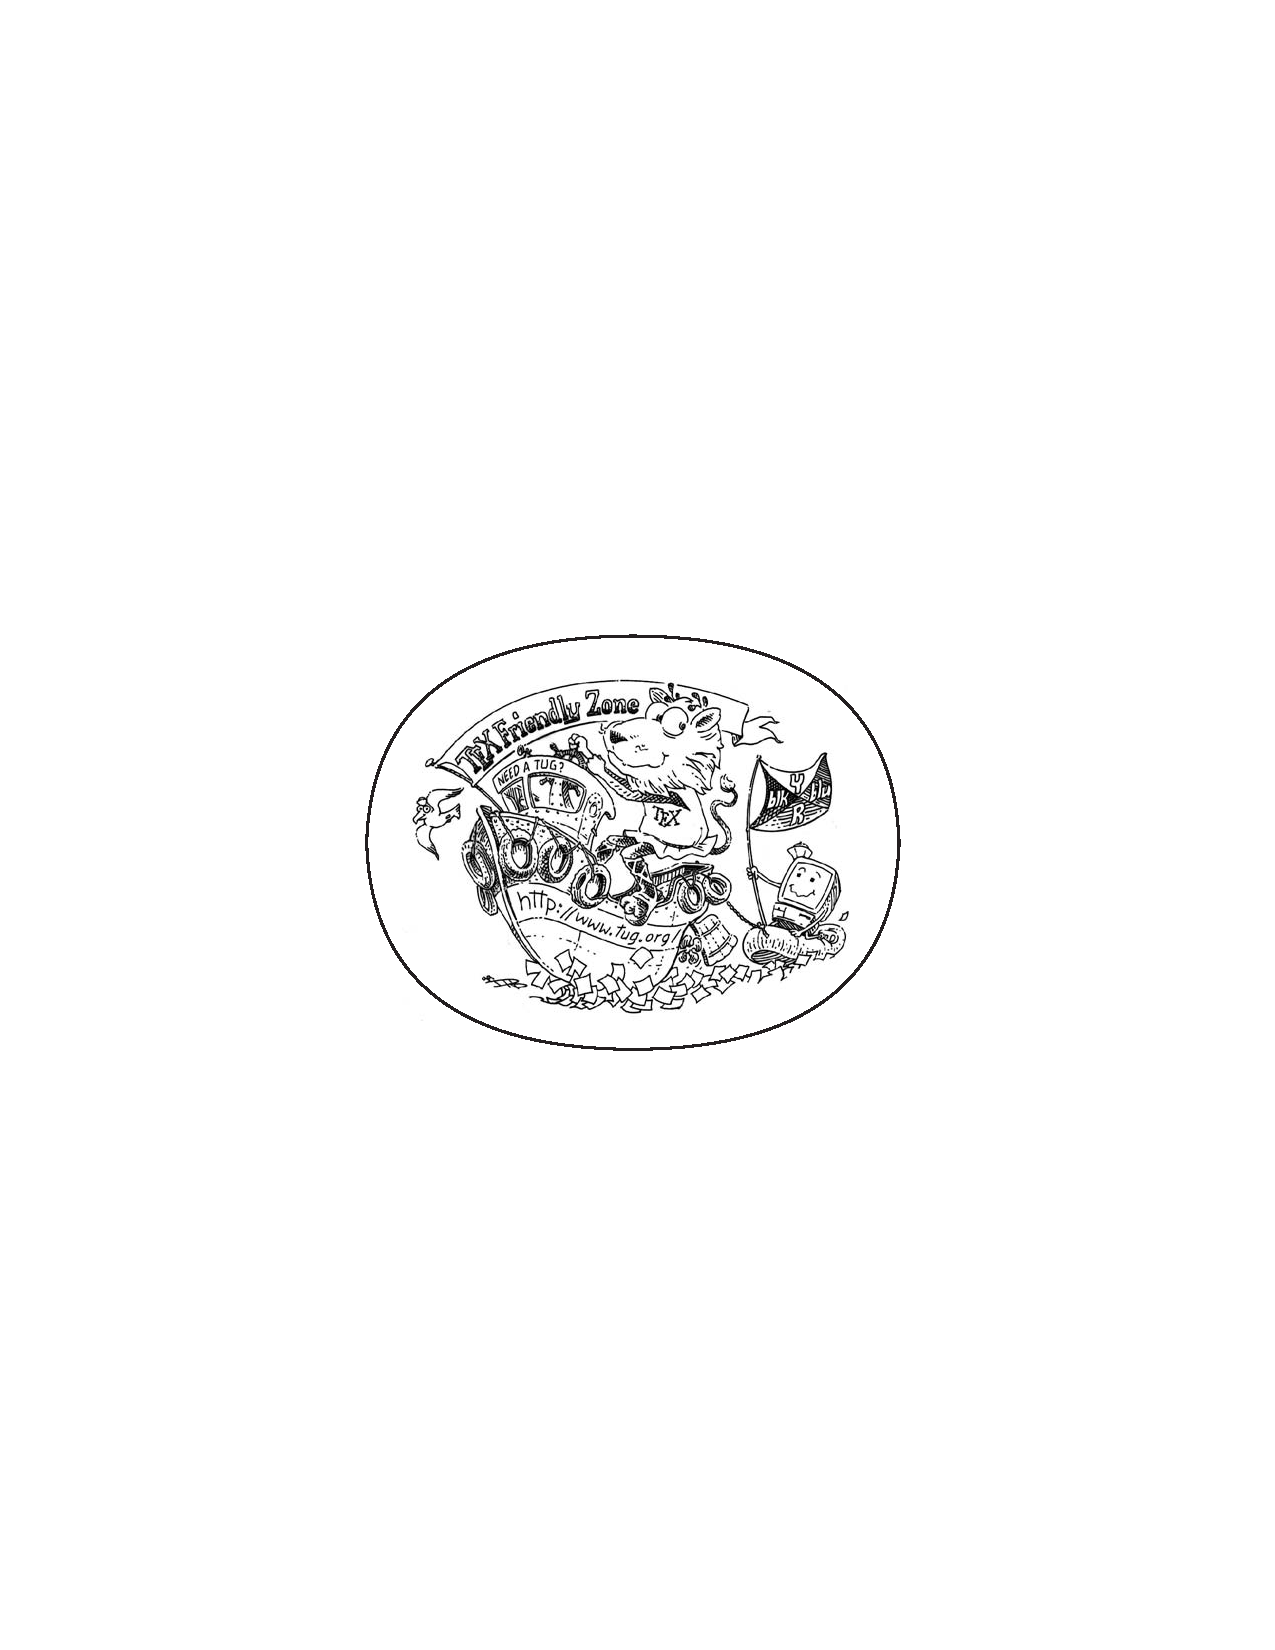
\includegraphics[width=6cm]{gfx/TFZsuperellipse_bw} \\ \medskip

        \mySubtitle \\ \medskip
        %\myDegree \\
        \myDepartment \\
        \myFaculty \\
        \myUni \\ \bigskip

        \myTime\ -- \myVersion

        \vfill

    \end{center}
  \end{addmargin}
\end{titlepage}

\thispagestyle{empty}

\hfill

\vfill

\noindent\myName: \textit{\myTitle,} \mySubtitle, %\myDegree,
\textcopyright\ \myTime

%\bigskip
%
%\noindent\spacedlowsmallcaps{Supervisors}: \\
%\myProf \\
%\myOtherProf \\
%\mySupervisor
%
%\medskip
%
%\noindent\spacedlowsmallcaps{Location}: \\
%\myLocation
%
%\medskip
%
%\noindent\spacedlowsmallcaps{Time Frame}: \\
%\myTime

\cleardoublepage%*******************************************************
% Dedication
%*******************************************************
\thispagestyle{empty}
\phantomsection
\pdfbookmark[1]{Dedication}{Dedication}

\vspace*{3cm}

\begin{center}
      This thing is complex... so complex not even God gets it.\\ \medskip
    --- Rafa Buscalioni
    \\ \medskip\medskip
        There is no way you are getting a quote for your stupid thesis\\ \medskip
    --- NVIDIA

\end{center}

\medskip

%\cleardoublepage\input{FrontBackmatter/Foreword}
\cleardoublepage%*******************************************************
% Abstract
%*******************************************************
%\renewcommand{\abstractname}{Abstract}
\pdfbookmark[1]{Abstract}{Abstract}
% \addcontentsline{toc}{chapter}{\tocEntry{Abstract}}
\begingroup
\let\clearpage\relax
\let\cleardoublepage\relax
\let\cleardoublepage\relax

\chapter*{Abstract}

Some abstract


\cleardoublepage%*******************************************************
% Publications
%*******************************************************
\pdfbookmark[1]{Publications}{publications}
\chapter*{Publications}
The following publications resulted from the development of this work
%\noindent Put your publications from the thesis here. The packages \texttt{multibib} or \texttt{bibtopic} etc. can be used to handle multiple different bibliographies in your document.

\begin{refsection}[ownpubs]
    \small
    \nocite{*} % is local to to the enclosing refsection
    \printbibliography[heading=none]
\end{refsection}

\cleardoublepage%*******************************************************
% Acknowledgments
%*******************************************************
\pdfbookmark[1]{Acknowledgments}{acknowledgments}

\begin{flushright}{\slshape}
\end{flushright}



\bigskip

\begingroup
\let\clearpage\relax
\let\cleardoublepage\relax
\let\cleardoublepage\relax
\chapter*{Acknowledgments}

\cleardoublepage%*******************************************************
% Table of Contents
%*******************************************************
\pagestyle{scrheadings}
%\phantomsection
\pdfbookmark[1]{\contentsname}{tableofcontents}
\setcounter{tocdepth}{2} % <-- 2 includes up to subsections in the ToC
\setcounter{secnumdepth}{3} % <-- 3 numbers up to subsubsections
\manualmark
\markboth{\spacedlowsmallcaps{\contentsname}}{\spacedlowsmallcaps{\contentsname}}
\tableofcontents
\automark[section]{chapter}
\renewcommand{\chaptermark}[1]{\markboth{\spacedlowsmallcaps{#1}}{\spacedlowsmallcaps{#1}}}
\renewcommand{\sectionmark}[1]{\markright{\textsc{\thesection}\enspace\spacedlowsmallcaps{#1}}}
%*******************************************************
% List of Figures and of the Tables
%*******************************************************
\cleardoublepage
% \pagestyle{empty} % Uncomment this line if your lists should not have any headlines with section name and page number
\begingroup
    \let\cleardoublepage\relax
    \let\cleardoublepage\relax
    %*******************************************************
    % List of Figures
    %*******************************************************
    %\phantomsection
    %\addcontentsline{toc}{chapter}{\listfigurename}
%    \pdfbookmark[1]{\listfigurename}{lof}
%    \listoffigures

    \vspace{8ex}

    %*******************************************************
    % List of Tables
    %*******************************************************
    %\phantomsection
    %\addcontentsline{toc}{chapter}{\listtablename}
    \pdfbookmark[1]{\listtablename}{lot}
    \listoftables

    \vspace{8ex}
    % \newpage

    %*******************************************************
    % List of Listings
    %*******************************************************
    %\phantomsection
    %\addcontentsline{toc}{chapter}{\lstlistlistingname}
    \pdfbookmark[1]{\lstlistlistingname}{lol}
    \lstlistoflistings

    \vspace{8ex}

    %*******************************************************
    % Acronyms
    %*******************************************************
    %\phantomsection
    \pdfbookmark[1]{Acronyms}{acronyms}
 %   \markboth{\spacedlowsmallcaps{Acronyms}}{\spacedlowsmallcaps{Acronyms}}
%    \chapter*{Acronyms}
    \printglossary[type=\acronymtype]
\endgroup


\cleardoublepage
\pagestyle{scrheadings}
\pagenumbering{arabic}
%\setcounter{page}{90}
% use \cleardoublepage here to avoid problems with pdfbookmark
\cleardoublepage
\part{Introduction}\label{pt:intro}
\chapter{Introduction}\label{ch:introduction}


The modeling and simulation of physical systems is always tied to a certain spatio-temporal scale. More often than not, studying a system through the lens of a certain scale prevents the exploration of the others.
Choosing the right lens for a problem requires understanding of its characteristic times and lengths.
Say, for instance, that you want to study the caudal of a waterfall throughout the next thousand years. It would be a bad decision to employ quantum mechanics for such a feat, a theoretical framework best suited for events that take femtoseconds and are measured in angstroms.
A lot of mathematical frameworks and numerical techniques are known for the exploration of different spatio-temporal scales. However, some times the need arises to tackle a phenomenon that unravels between their scope.
On the other hand, the advent of supercomputing in the last two decades has presented the field with new powerful tools to leverage. For the first time we have more computing power than what our techniques are capable of handling. 
Developing new techniques (numerical and theoretical) directly aimed to these new techonologies will allow to explore regimes previously unreachable, opening the doors to a world of secrets waiting to be found.
The fields that can take advantage of more computing power the most are those that mix several spatio-temporal regimes.
For instance, when we need to simulate every molecule of a virus capsid submerged in water for a very long time\cite{virusfullatom2018}. In this article, the authors simulate the dynamics of $6$ million atoms (explicitly) in the span of $1\mu s$, requiring $5 10^8$ simulation steps.
Of course, this kind of simulation would be impossible without the aid of a super computer and a family of software tools to take advantage of it.
This thesis is devoted to the development of new algorithms and software tools for the study of complex fluids and biological systemsin high performance computing environments. It just so happens that the interesting physics of these processes often lie in this intermediate regime, called the \emph{mesoscale}.
The definition of mesoscale is kind of fuzzy, but mesoscopic physics normally deal with entities ranging from $50-100nm$ (a typical virus) to $~10\mu m$ (the size of a HeLa cell), with characteristic times going from a few micro seconds to even minutes.
The mesoscale poses a series of theoretical and numerical challenges, stemming from the wide range of spatio-temporal scales that influence them. A perfect fit for a super computer.
Another example of this kind of simulations is the one described in \cite{fullatombacteria2016}. In this article the authors employ $100$ million particles to simulate a chunk of the interior environment of a bacteria for some tens of nanoseconds (around $10^7$ steps).

Recently, a new paradigm of supercomputing has arisen. The \gpu, a massively parallel copocressor. So powerful that it requires to straight-up rethink our algorithms to take advantage of it.
\todo{continue}
%\begin{figure}
%  \label{fig:landscape}
%  \centering
%%  \begin{tikzpicture}
%%    \begin{loglogaxis}[
%%      width=\textwidth,
%%      height=\axisdefaultheight,
%%      xmin=1e-11,xmax=100,
%%      xtick={1e-10, 10e-9, 1e-6, 1e-3, 1, 100},
%%      xticklabels={0.1 nm, 10 nm, 1 $\mu$m, 1 mm, 1 m, 100 m},
%%      ymin=1e-15,ymax=86400,
%%      ytick={1e-15, 1e-12, 1e-9, 1e-6, 1e-3, 1, 3600, 86400},
%%      yticklabels={1 fs, 1 ps, 1 ns, 1 $\mu$s, 1 ms, 1 s, 1 h, 1 day}
%%      ]
%%      \addplot[color=red, domain=1e-11:100 ]{1000000*x^2.5};
%%    \end{loglogaxis}
%%  \end{tikzpicture}
%  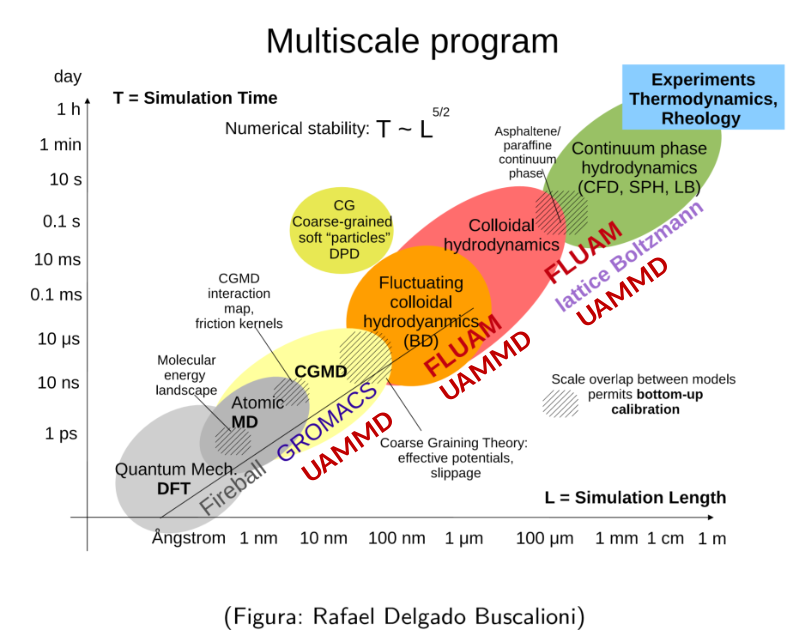
\includegraphics[width=\textwidth]{landscape}
%  \caption{A landscape of numerical techniques}
%\end{figure}

\section{The Graphical Processor Unit}

The \gpu technology, interpreted as some kind of specialized graphic circuit or co-processor, can be tracked back to the 1970s. Once electronic devices started having screens attached to them, it made sense to have some kind of chip translating the CPU information into the analogic signal of the display. It was then only a matter of time before more functionality was put into them. It started as a way to accelerate the display process in early video game hardware, such as arcade systems.
Storing the data that goes into the screen takes a lot of space and, at the time, RAM memory was expensive (still is, by the way!).

In 1977, the Atari 2600 (one of the first home consoles) could simply not afford to store the contents of its 160x80 pixel display into its 128 bytes of RAM. Of course, these systems employed some truly creative software tricks to reduce memory usage. However, the numbers just do not add up. Even if we limit ourselves to a monochrome output (so one pixel takes one bit to store), the frame buffer for a 160x80 pixel display takes 1600 bytes\footnote{In contrast, the NVIDIA GTX 980 (the trusty, consumer-grade, GPU that has accompanied my thoughout most of my Ph.D.) has 4 GB of memory and will happily output to a several screens with 4k resolution (4096x2160 pixels).}.
The solution was to not have a frame buffer at all, rather outsource the display operations to a specialized hardware. The Atari 2600's graphic chip had a 128 color palette and allowed developers to use close to 5 sprites to design their 2D games.

These chips were little more than video display chips, but they were the predecesors to the \gpu.
Throughout the next decade the hardware evolves to support faster and more complex operations, hold more memory, etc. In 1990 a graphic adaptor could draw 16 million different colors to a 1028x1024 pixel display and hold 1MB of data.

Graphic adaptors were still centered around 2D graphic acceleration, such as graphical user interfaces and 2D games. However, the market was already pushing for real-time 3D graphics in games. Although one could hack the current 2D graphic pipeline to draw 3D environments, without specialized hardware acceleration (as was already common for 2D) the results were far from interactive. Surely it would be a task best suited for the graphic adaptor technology already established.

Soon enough, during the early and mid 1990s, several companies were releasing their graphic adaptors with 3D acceleration capabilities. In 1994 the term \gpu is coined to designate this hardware, which had evolved beyond its original task of just sending pixels to a display.
OpenGL\cite{opengl}, one of the first graphics \gls{API}\footnote{A software library.}, appears in the early 1990s attempting to standardize the programming of graphic hardware accelerators, specially for 3D.
At the time OpenGL had quite limited capabilities, allowing a developer to do little more than to feed a fixed pipeline with triangles. OpenGL would then interface with the \gpu to turn this geometry into a 2D image that could be displayed.
Naturally this translation involves a great deal of raw computation, further transforming the \gpu from a video display card to an independent co processor. Furthermore the usual operations required to do this happen to be inherently parallel. While the CPU evolved to be formed by a single, powerful, core the \gpu was born out of a parallel computing necessity. Thus a \gpu tends to have many, less powerful, processing cores.
Jumping again to the year 2000 the quality and complexity of computer graphics has exploded. Card manufacturers have included all sorts of new 3D hardware accelerated operations beyond simple triangles. And OpenGL has evolved along them. As it usually happens people have started to hack around, using the graphics pipeline to perform computations not necessarily related to computer graphics. In particular, a new \gpu was presented by the NVIDIA Corporation in 2001 that allowed to modify the different stages of the graphic pipeline via something called programmable shaders. These shaders were short programs that could intercede between the different stages of drawing. A vertex shader could be written to process each triangle before sending it to a fragment shader, which could process each pixel on the screen before finally sending them to the display. This was the advent of the so-called \gls{GPGPU}.

Shaders were enough for the community to realize that drawing polygons was far from the only thing they could do with a \gpu\cite{gpgpu2002}. Applications exploting shaders arise everywhere in a variety fields like scientific image processing \cite{gpuimage2003, gpuimage2006}, lineal algebra \cite{gpulinalg2001, gpulinalg2003a, gpulinalg2003b}, physics \cite{gpulbm2004} and even machine learning\cite{gpuml2005, gpuml1998}. One can even find a molecular dynamics code running on the \gpu of a Sony PlayStation 3 \cite{ps3md2009}.

The next natural step took place in 2007, when the NVIDIA Corporation released CUDA\cite{cuda}.
\begin{figure}
  \centering
  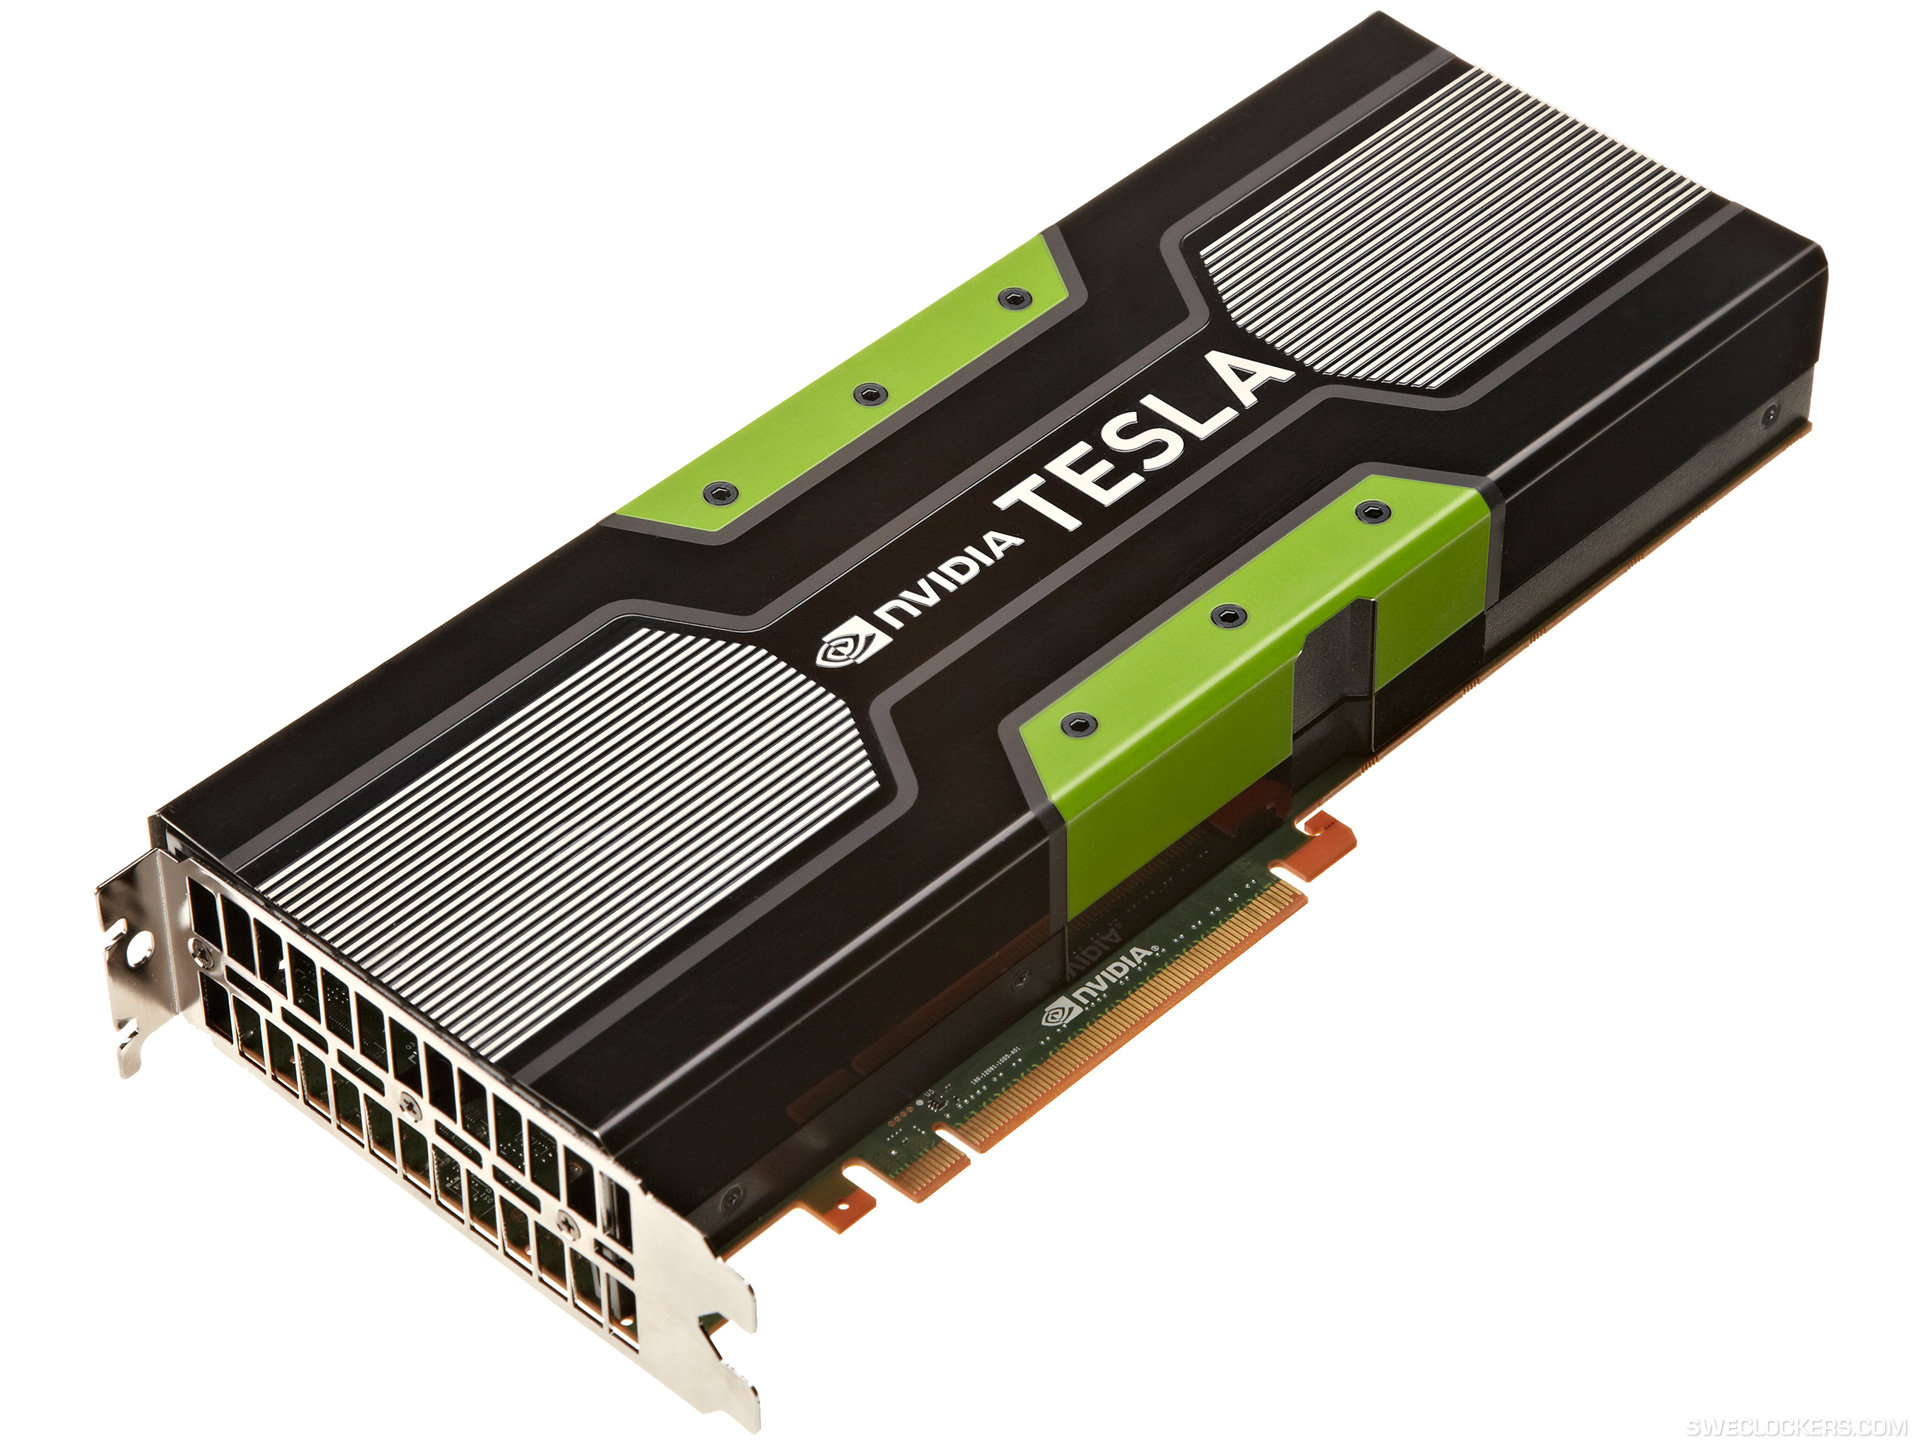
\includegraphics[width=\textwidth]{gpu_and_me}
  \caption{A picture of the author with a GPU ( a NVIDIA's RTX 2080Ti ).}
  \label{fig:gpuandme}
\end{figure}
\todo{continue}
\section{Software for soft matter simulations}
Problems with porting CPU centric \gls{MD} packages to \gpu. Scalability in software.

Many \gls{MD} software projects started at a time when the \gpu was not a widespread tool for general computing (or did not even existed as hardware). Take for example GROMACS \cite{gromacs}, which was born in 1991

The present and future of high performance computing.
CUDA vs alternatives.

Scientific computing in the GPU era.

Developing algorithms for the ground up with the GPU architecture in mind is essential. Leverage ultra efficient \gpu \gls{FFT} by developing spectral algorithms. Many times simplicity beats complexity.

State of the art in molecular simulations.
\todo{continue}

\cleardoublepage
\ctparttext{Description of the UAMMD infrastructure. Importance of fundamentally GPU-driven design.}
\part{UAMMD: Design and components}\label{pt:uammd}
%*****************************************
\chapter{Design principles}\label{ch:design}
\todo{FILL}
Open infrastructure instead of closed ecosystem. Open source. C++, header only.
\section{Universality}
Anything goes as long as it has interacting entities. One could technically implement Chess as a module.
\section{Adaptability}
Highly templated code and super generic interfaces. 
\section{Mulstiscale}
From atoms in vacuum to chunks of oceans and planetary dynamics.
\section{Molecular Dynamics}
Using molecular in the sense of an arbitrarily coarsed-grained simulation unit (atoms, groups of atoms, colloids, groups of colloids, buckets of water, planets...)

\chapter{Core Components}\label{ch:core}
How the design principles are exposed in code. \todo{FILL}
\section{System}
\todo{FILL}
\section{ParticleData}
\todo{FILL}
\section{ParticleGroup} 

\todo{FILL}


%\chapter{Algorithms}\label{ch:algorithms}
%Algorithms in the basic \gls{UAMMD} infrastructure. 
%\section{Cell List}
%No need to really construct a neighbour list, reference  to Transverser
%\section{Verlet List}
%mostly obsolete thanks to cell list
%\section{Bonded Forces}
%Bonded Forces as a kind of neighbour list
%\section{IBM}\label{ch:ibm}
%Change to something more meaningful that conveys spreading+interpolation
%

%\chapter{Interfaces}\label{ch:interfaces}
%This stuff should go organically in the text
%Generic interfaces desgined to communicate with the core \gls{UAMMD} componentes.
%\section{Transverser}
%The Transverser interface. Transform + traverse
%\section{Potential}
%To encapsulate Transversers
%\section{ParameterUpdatable}
%An interface to communicate changes in parameters
%

\chapter{Usage examples throughout this document}\label{sec:uammd_struct}
Every time an algorithm available in \uammd is presented it will be acompanied by a section describing how to use it in the codebase.
Often this will consist of a function creating and returning an instance of the related module in the following form


\begin{minted}{\ucpp}
#include<uammd.cuh>
//Additional includes when necessary
using namespace uammd;
auto createModule(UAMMD sim){
//Some preparation...
return std::make_shared(Module(/*Whatever is needed*/));
}
\end{minted}

These examples are meant to serve both as a tutorial and an easily copy-pastable example.
The structure \emph{UAMMD} in these examples is not part of \uammd and is meant to group the core components of a typical \uammd code. It can be defined as follows


\begin{minted}{\ucpp}
#include<uammd.cuh>
//Additional includes when necessary
using namespace uammd;
//An aggregate of parameters required by the relevant modules in the code
struct Parameters{
  //real dt;
  //...
};
struct UAMMD{
  std::shared_ptr<System> sys;
  std::shared_ptr<ParticleData> pd;
  std::shared_ptr<ParticleGroup> pg;
  Parameters par;
};

//A function creating an instance of the UAMMD structure
UAMMD initializeUAMMD(){
  UAMMD sim;
  Parameters par;
  //Fill out parameters somehow
  //par.dt = 0.1;
  sim.par = par;
  sim.sys = std::make_shared<System>();
  //Set the number of particles some how.
  int numberParticles = 1e6;
  sim.pd  = std::make_shared<ParticleData>(sys, numberParticles);
  //A group with all the particles.
  sim.pg = std::make_shared<ParticleGroup>(pg, sys, "All");
  return sim;
}
\end{minted}

\section{Error handling in UAMMD}\label{sec:uammd_errors}
Errors are communicated via C++ exceptions.

Examples

\todo{FILL}

\section{Basic concepts of GPU programming}
\todo{FILL}
Things to explain here:

Different memories; Separation between CPU and GPU RAM, global memory, register memory, shared memory, constant memory.

\part{A voyage through numerical space-time}

Let us go through the different numerical techniques that are used to simulate the different sections of the spatio-temporal landscape.

\begin{figure}
  \centering
  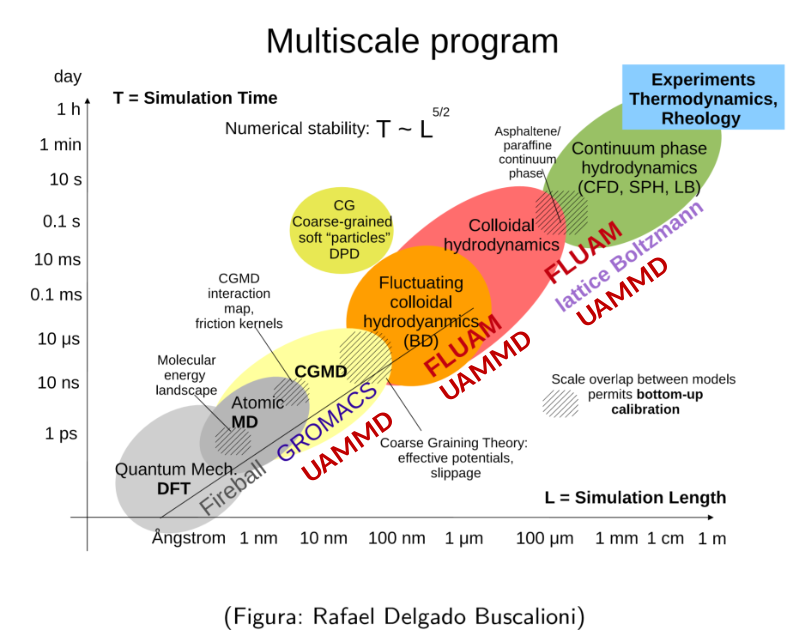
\includegraphics[width=\textwidth]{landscape}
  \caption{The spatio-temporal landscape and its numerical techniques.}
  \label{fig:sptime-land}
\end{figure}
\todo{RAFA, te he fusilado esta img que me gusta mucho. Me gustaria rehacerla solo con lo que me interesa, pero me esta costando encontrar referencias}

We can distinguish between two families of numerical techniques, particle and grid based methods. The second one also uses particles, but the heavyweight of the algorithm is carried out in a grid, as apposed to just the positions of the particles.
In some way or another, all algorithms have to take into account interactions between particles.

\chapter{Working with particles}
Let us interpret the word \emph{particle} as a relatively small discrete portion in a simulation. This is a vage definition on porpuse, since from an algorithmic point of view it does not really matter what a particle represents. Sometimes a particle will be an atom or molecule, other times it will make more sense that our simulation unit is a big colloid, a virus or a whole sun.
The important thing about particles is that when several of them are present, they more than often have a certain effect on each other.
Stars in a galaxy attract each other over an infinetely long range of space, while two argon atoms will repell each other at close range.
Even if particles are somehow oblivious to each other, they might interact with some other thing, like fluid particles being repelled by a wall.
Each kind of interaction requires a different approach, and figuring out how to efficiently compute it in a \gpu is a field on itself. 
In this chapter we will see some of the strategies that can be employed and how they are implemented in \uammd.

\chapter{Particle interactions}


Let us see how \uammd deals with interactions by introducing the \emph{Interactor} module.

\section{The Interactor interface} \label{sec:interactor}

Interactor encapsulates the concept of a group of particles interacting, be it with each other or with some external influence.
An Interactor can be issued to compute, for each particle, the forces, energies and/or virial due to a certain interaction.
To do so it can access the current state of the particles (like positions, velocities, etc).
A minimal example of an Interactor

\begin{minted}{\ucpp}
#include<uammd.cuh>
#include<Interactor/Interactor.cuh>
using namespace uammd;

//A class that needs to behave as 
//an UAMMD Interactor must inherit from it
class MyInteractor: public Interactor{
public:
  MyInteractor(shared_ptr<ParticleData> pd,
               shared_ptr<ParticleGroup> pg,
               shared_ptr<System> sys):
          Interactor(pd, pg, sys, "MyInteractor"){
    //Any required initialization 
  }

  virtual void sum(Computables comp, cudaStream_t st){
    if(comp.force){
      //Sum forces to each particle
    }
    if(comp.energy){
      //Sum energies to each particle
    }
    if(comp.virial){
      //Sum virial to each particle
    }
  }
};
\end{minted}

See chapter \ref{ch:core} for information about how to access particle properties and using particle groups.

\uammd offers a series of \emph{Interactors} with the different kinds of interactions that we will discuss in the following sections. Sometimes exposing a general algorithm that can be specialized (like \emph{PairForces} for particle pair interactions, see sec. \ref{sec:pairforces}) and others exposing particular potentials (like \emph{SpectralEwaldPoisson} for electrostatics, see sec. \ref{sec:tppoisson}).

It is also worth introducing here two other interfaces that \uammd uses to work with particles, \emph{Transverser} and \emph{Potential}.

\section{The Transverser Interface} \label{sec:transverser}
A Transverser is a concept that refers to the action of going through each element of something.  

For example, for each particle, we want to perform some computation for particles that are closer than a certain distance in a custom way. Or more generally, we want to perform some kind of operation equivalent to a matrix-vector multiplication, for which in order to compute one element of the result, the vector needs to go through a row of the matrix.
In these cases, a Transverser is used.

A Transverser holds information about what to do with a pair of particles, what information is needed to compute this interaction, or what to do when a particle has interacted with all pairs it is involved in.  

Being such a general concept, a \emph{Transverser} is used as a template argument, and therefore cannot be a base virtual class that can be inherited. This is why it is a "concept". No assumption can be made about the return types of each function, or the input parameters, the only things general are the function names.  

For each particle to be processed the \emph{Transverser} will be called for:  
\begin{itemize}
\item Setting the initial value of the interaction result (function \emph{zero})
\item Fetching the necesary data to process a pair of particles  (function \emph{getInfo})
\item Compute the interaction between the particle  and each of its neighbours (function \emph{compute})
\item Accumulate/reduce  the result for each neighbour (function \emph{accumulate})
\item  Set/write/handle the accumulated result for all neighbours (function \emph{set})
 \end{itemize}
The same Transverser instance will be used to process every particle in an arbitrary order. Therefore, the Transverser must not assume it is bound to a specific particle.

The \emph{Transverser} interface requires a given class/struct to provide the following public device (unless prepare that must be a host function) member functions:

\begin{itemize}
\item \mintinline[breaklines]{\ucpp}{Compute compute(real4 position_i, real4 position_j,Info info_i, Info info_j);}

  
  For a pair of particles
  characterized by position and info this function must return the
  result of the interaction for that pair of particles. The last
  two arguments must be present only when \emph{getInfo} is defined.The
  returning type, \emph{Compute}, must be a POD type (just an aggregate of
  plain types), for example a real when computing energy.

\item \mintinline{\ucpp}{void set(int particle_index, Compute &total);}

  
   After calling compute for all neighbours this function will be called with the contents of "total" after the last call to "accumulate".
   Can be used to, for example, write the final result to main memory.

 \item \mintinline{\ucpp}{Compute zero();}

   
   This function returns the initial value of the computation, for example {0,0,0} when computing the force. 
   The returning type, \emph{Compute}, must be a POD type (just an aggregate of plain types), for example a real when computing energy. Furthemore it must be the same type returned by the "compute" member.
   This function is optional and defaults to zero initialization (it will return Compute() which works even for POD types).
    
 \item \mintinline{\ucpp}{Info getInfo(int particle_index);}

   
   Will be called for each particle to be processed and returns the per-particle data necessary for the interaction with another particle (except the position which is always available). For example the mass in a gravitational interaction or the particle index for some custom interaction.
   The returning type, Info, must be a POD type (just an aggregate of plain types), for example a real for gravitation.
   This function is optional and if not present it is assumed the only per-particle data required is the position. 
   In this case the function "compute" must only have the first two arguments.

 \item \mintinline{\ucpp}{void accumulate(Compute &total, const Compute &current);}

   
  This function will be called after "compute" for each neighbour with its result and the accumulated result.
  It is expected that this function modifies "total" as necessary given the new data in "current".
  The first time it is called "total" will be have the value as given by the "zero" function.
  This function is optional and defaults to summation: total = total + current. Notice that this will fail for non trivial types.
     
\item \mintinline{\ucpp}{void prepare(std::shared_ptr<ParticleData> pd);}

  
  This function will be called one time in the CPU side just before processing the particles.
  This function is optional and defaults to simply nothing.
 \end{itemize}

Lets see a trivial example.
This \emph{Transverser} can be used with a neighbour list to count the number of neighbours of each particle:
\begin{listing}
\begin{minted}{\ucpp}
struct NeighbourCounter{
  int *nneigh;
  real rc;
  Box box;
  NeighbourCounter(Box i_box, real i_rc,int *nneigh):
    rc(i_rc),box(i_box),
    nneigh(nneigh){}

  //There is no "zero" function so the total result starts being 0.
  
  //For each pair computes counts a neighbour 
  //if the particle is closer than rcut
  __device__ int compute(real4 pi, real4 pj){
    const real3 rij = box.apply_pbc(make_real3(pj)-make_real3(pi));
    const real r2 = dot(rij, rij);
    if(r2>0 and r2< rc*rc){
      return 1;
    }
    return 0;
  }
  //There is no "accumulate"
  // the result of "compute" is added every time.
  //The "set" function will be called with the accumulation
  // of the result of "compute" for all neighbours. 
  __device__ void set(int index, int total){
    nneigh[index] = total;
  }
};
\end{minted}
\caption{A \emph{Transverser} that counts the number of neighbours of each particle}
\label{code:ncounter}
\end{listing}
In the following sections, we will see how to use \emph{Transversers} to compute forces, energies and more between particles.
But in order to do that, we need yet another interface in order connecting the general concept of a \emph{Transverser} with something that computes forces, energies or virial of an interaction. In \uammd, we use the \emph{Potential} interface for that.

\section{The Potential Interface} \label{sec:potential}

This interface is just a connection between the \emph{Transverser} and \emph{Interactor} concepts. Additionally, \emph{Potential} aids with one limitation of the CUDA programming language and \gls{GPU} programming in general. On one hand, register memory in a \gpu is quite limited, so it is not a good idea to use large objects in a kernel. On the other hand there are some technical details that prevents certain objects from existing in a \gpu kernel. For example, objects are passed by value to a kernel, which can incurr in undesired copies and/or destructors being called. Thus, its some times worth it to make a conceptual and programmatic separation between CPU and \gpu objects.
In this regard, \emph{Transversers} are \gpu objects, while \emph{Interactors} or \emph{Potentials} are meant to be used in the CPU.
Furthermore, while \emph{Transverser} describes a very general computation, \emph{Potential} only holds the logic on how to compute forces, energies and/or virials.
\emph{Potential} serves as a way to serve \emph{Transversers} to \emph{Interactors}.

\todo{DESCRIBE INTERFACE}





We are now ready to start exploring the different types of particle interactions, mainly:
\begin{itemize}
\item Long range interactions
\item Short range interactions
\item Bonded interactions
\end{itemize}

Let us go through each of them and describe the different algorithms used to solve each case and how \uammd exposes them.


\section{Periodic Boundary Conditions}
In order to conserve the total volume of the system we use the \gls{MIC}, where a particle that leaves the simulation domain though one side appears on the other.
Numerically we can express this algorithm as follows:

\begin{algorithm}
  \caption{Minimum Image Convention, takes a position or distance and returns it inside the simulation domain}
  \begin{algorithmic}[1]
    \Function{MIC}{r, L}   
    \State \Return r - floor(r/L + 0.5)*L
    \EndFunction
  \end{algorithmic}
\end{algorithm}
We can also use this algorithm to get the minimum distance between two points, so particles near opposite walls interact.
\subsection{Use in UAMMD}
In \uammd, \gls{MIC} can be accesed via the \emph{Box} class.
\begin{listing}[H]
\begin{minted}{\ucpp}
#include<uammd.cuh>
using namespace uammd;
int main(){
  real lx, ly, lz;
  lx = ly = lz = 32.0;
  Box box({lx, ly, lz});
  real3 position_outside_box = {0.5*lx+1, 0, 0};
  real3 position_in_box = box.apply_pbc(position_outside_box);
  //position_in_box holds {-lx*0.5+1,0,0}
  return 0; 
}
\end{minted}
\caption{Using the Box class.}
\label{code:box}
\end{listing}
In \uammd the \emph{Box} object handles the domain details, including \gls{PBC}.
\todo{code example}



\section{Long range interactions}
Say we are set to simulate a galaxy, so far away from others that it can be safely assumed their action is negligible. Say we want to simulate the dynamics of each of the $N$ stars in this galaxy. Gravity is the dominating interaction between each star, sadly it decays slowly enough to be considered an infinitely ranged one. The gravity potential can be written as follows
\begin{equation}
  \label{eq:gravity}
  U(r) = G\frac{m_1m_2}{r}
\end{equation}
Where $G$ is the gravitational constant and $m_1$, $m_2$ are the masses of each particle.
In this case, if we want to compute the force acting on a star due to the presence of all the others we must check each and everyone of them. This leads to a lot of interactions to check, more precisely $N^2$ of them. Of course, there are more sophisticated ways of performing such a computation, such as fast multipole methods \cite{fmm} or Ewald splitting (which will be discussed on section \ref{ewald}). But some times these techniques are not a possibility so it is valuable to see how to efficiently handle this computations.
Furthermore this computation is a really good fit for a \gls{GPU} as we are going to see.
\subsection{The NBody algorithm}
The naive parallel algorithm that checks, for each particle, every other would simply assign a particle (or a group of them) to a thread and then iterate over the rest is summarized in algorithm \ref{alg:nbodynaive}.
\begin{algorithm}
  \caption{Naive NBody algorithm. Each particle, i, visits all the others.}\label{alg:nbodynaive}
  \Input{A list of $N$ particles}
  \begin{algorithmic}[1]
    \Require A thread is launched per particle    
    \State $i \gets$ thread ID \Comment{Particle index}
    \For{ $j=0$ until $N$}
    \LeftComment{Process $i$-$j$ pair}
    \EndFor
  \end{algorithmic}
\end{algorithm}
This is an embarrasingly parallel operation in which, in principle, a thread can work without collaborating with the others. However the naive algorithm is missing an oportunity in doing so. We can leverage that all threads have to access the same segments of memory. Instead of letting each thread diverge we can enforce that all threads access the same particles at the same time. This can effectively reduce the number of global memory acceses to a certain particle from $N$ to, potentially, just one.
This algorithm is based on the \emph{nbody} algorithm originally devised by NVIDIA\cite{nbody1,gpugems3,cudahandbook}. It leverages the shared memory capabilities of the \gpu by assigning a thread to a particle and then collaboratively loading groups of particles (called tiles) into shared memory. Then each thread processes this tile loaded into shared memory. This is repeated until all tiles have been loaded and processed.
The optimal size of a tile will be an optimization parameter also depending on the required shared memory per particle, being the number of threads in a block (or a multiple of it) a good default.
This results in an overall speedup of 30 compared with the naive algorithm \todo{Maybe a figure comparing here?}
The algorithm is summarized in algorithm \ref{alg:nbody}-
\begin{algorithm}
  \caption{Shared memory NBody algorithm GPU kernel. Although the number of particles per tile is unconstrained, for simplicity this pseudocode assumes a tile has a size equal to the number of threads per block, with a number of tiles equal to the number of thread blocks.} \label{alg:nbody}
  \Input{A list of $N$ particles}
  \begin{algorithmic}[1]
    \Require
    \Statex A group of $N_b$ thread blocks with $N_{th}$ threads per block is launched.
    \Statex At least a thread per particle.
    \Statex Enough shared memory per block to to store $N_{th}$ particles.
    \Ensure
    \Statex Threads with index larger than $N$ do not participate.
    \State i $\gets$ thread ID \Comment{The index of the particle asigned to this thread.}
    \State tid $\gets$ mod($i$, $N_{th}$) \Comment{Index of thread in the block.}
    \For{tile $=0$ until $N_b$}
    \State iload $\gets \text{tile } N_{th}+$tid
    \State Load particle \emph{iload} into shared memory at index \emph{tid}.
    \State Synchronize threads in block. \Comment{Ensures the entire tile is loaded.}
    \For{counter $ =0$ until $N_{th}$}
    \State $j \gets \text{tile }N_{th} + \text{counter}$
    \State Read particle $j$ from shared memory index \emph{counter}.
    \State{Process $i$-$j$ pair}
    \EndFor
    \State Synchronize threads in block. \Comment{Ensures shared memory can be rewritten}
    \EndFor
  \end{algorithmic}
\end{algorithm}

Note that the computation as described here is not restricted to computing forces or energies between particles, it might be used for widely different computations that can be encoded as an nbody operation.
\uammd acknowledges this generality via the \emph{Transverser} interface (see sec. \ref{sec:transverser}), that can be used to specialize these algorithms. 
\subsection{Use in UAMMD}
There are three ways to access this algorithm depending on the final usage.
The first is to use it to process a \emph{Transverser} acting on a group of particles:
\begin{minted}{\ucpp}
#include<uammd.cuh>
#include<Interactor/NBody.cuh>
using namespace uammd;
//For each particle, applies a Transverser with all other particles.
template<class Transverser>
void tranverseWithNBody(UAMMD sim, Transverser tr){
  NBody nb(sim.pd, sim.pg, sim.sys);
  //Optionally, the function can run on a cuda stream
  cudaStream_t st = 0;
  nb.transverse(tr, st);
}
\end{minted}
The next one is to use it as an \emph{Interactor} to compute forces, energies and/or virials. This is done by providing the \emph{PairForces} module with a \emph{Potential} with an infinite cut off distance.
\begin{minted}{\ucpp}
#include<uammd.cuh>
#include<Interactor/PairForces.cuh>
using namespace uammd;
template<class Potential>
auto createLongRangedForcesWithPotential(UAMMD sim, Potential tr){
  using PairForces = PairForces<Potential>;
  return std::make_shared<PairForces> pf(sim.pd, sim.pg, sim.sys, potential);
}
\end{minted}
We will come back to \emph{PairForces} in the following chapters, as it can also work with short ranged potentials.
Finally, we can access \emph{NBody} outside the \uammd ecosystem (without \emph{ParticleData}, \emph{System}, etc).
\begin{minted}{\ucpp}
#include<uammd.cuh>
#include<Interactor/NBodyBase.cuh>
using namespace uammd;
template<class Transverser>
void transverseWithoutUAMMD(real4* positions, int numberParticles,
                            Transverser tr){
  NBodyBase nb;
  //Optionally, the function can run on a cuda stream
  cudaStream_t st = 0;
  nb.transverse(positions, tr, numberParticles, st);
}
\end{minted}




\section{Short range interactions}
Particles interacting closely, a.i. there is less information to share between them, allow for specific optimizations abusing the locality of the required computation.
In reality it can happen that the effect of one particle on another is short ranged in nature, as could be the case for interactions stemming directly from quantum effects such as Van-der-Walls forces. It can also happen that a combination of several long ranged interactions result in an effective short ranged one, such as a screened electrostatic interaction (like the DLVO potential). Other times when the interaction cannot be made to decay rapidly using natural arguments we can still transform it into a short range one with techniques such as Ewald splitting, which will be discussed in section \ref{sec:ewald}.
The reason for giving short range interactions so much credit is simple: Imagine a system with $N$ uniformly distributed particles inside a given domain. If we let each particle interact with every other we need to check $N^2$ pairs of particles as we already saw. On the other hand, restricting the interaction to a certain distance, such that each particle has a number of neighbours $k<<N$ reduces the number of checks to $kN$.

\subsection{The Lennard-Jones potential}
A standard potential employed to model the short range Van-der-Waals interactions is the Lennard-Jones potential \cite{lj} (\gls{LJ} for short). A rapidly decaying repulsive radial potential with an attractive tail.
\begin{equation}
  \label{eq:lj}
  U_{LJ}(r) = 4 \epsilon \left[ \left(\frac{\sigma}{r}\right)^{12} - \left( \frac{\sigma}{r}\right)^6 \right] 
\end{equation}
Which results in this expression for the force at a certain distance $\vec{r}$ between two points
\begin{equation}
  \label{eq:ljf}
  \vec{F}_{LJ}(\vec{r}) = -\nabla_{\vec{r}} U_{LJ} = 24 \epsilon \left[ \left(\frac{\sigma}{r}\right)^{7} - 2\left( \frac{\sigma}{r}\right)^{13} \right] \hat{\vec{r}}
\end{equation}
Where $r = ||\vec{r}||$ is the modulus of the distance vector and $\hat{\vec{r}}$ is an unit vector in the direcion of $\vec{r}$.
\begin{figure}
  \centering
  \includegraphics[width=\textwidth]{lj}
  \caption{The Lennard-Jones potential described in eq. \ref{eq:lj}}
  \label{fig:lj}
\end{figure}

Given the rapidly decaying nature of this otherwise infinite range potential it is standard to truncate it at a certain distance, usually $r_{cut} = 2.5\sigma$. At this distance the potential has a value of $U_{LJ}(r = r_{cut}) = -0.0615\epsilon$.
Ignoring the long range effects of this potential changes the equation of state of a \gls{LJ} fluid in a way that is well understood and tabulated\cite{ljtrunc}. By doing this we can devise more efficient algorithms that only need to take into account short range interactions.
Finally, in order to avoid jumps in the energy it is also standard to shift the potential in addition to this truncation. This is refered as the truncated and shifted Lennard-Jones potential
\begin{equation}
  \label{eq:ljts}
  U_{LJTS}(r) =
  \begin{cases}
      U_{LJ}(r) - U_{LJ}(r_{cut}) & r<r_{cut}\\
      0 & r\ge r_{cut}\\                                    
    \end{cases}
\end{equation}
The expression for the force remains as in eq. \eqref{eq:ljf}, simply truncated at $r=r_{cut}$.

Sometimes we are only interested in the repulsive part of the LJ potential, as a way of modelling hard spheres. In order to do so we truncate eq. \eqref{eq:lj} at its minimum, located at a distance $r_m = 2^{1/6}\sigma$, where $U_{LJ} = 0$. The resulting potential is called Weeks-Chandler-Andersen, or WCA, potential. We will refer to to it as $U_{WCA}$.
Often the parameters in eq. \eqref{eq:lj} will be used as natural units of energy, $\epsilon$ and length $\sigma$.
\subsection{Neighbour Lists}\ref{sec:nlist}
Imagine a system composed of an uniform distribution of argon atoms, whose interaction can be qualitatively modeled via the \gls{LJ} potential. When we talked about computing the gravitational interaction between stars, it made sense to devise an efficient algorithm that checks all star pairs in the system. However, in this new system governed by eq. \eqref{eq:ljts}, checking all pairs becomes pointless given that the vast mayority of them will contribute zero to the final result. We would like to skip all these pairs that lie beyond a certain cut off distance, $r_{cut}$, beforehand. A neighbour list contains, for each particle, a list of other particles that are closer than $r_{cut}$ to it. There are many approaches, wildly different between them, to constructing neighbour list, and \uammd implements several of them as we will shortly see.
Once a list is constructed, the traversal algorithm depends on the type of neighbour list. However, the logic behind traversal will always be the same (see algorithm \ref{alg:nlist}) and compatible with the \emph{Transverser} interface (which is actually the main reason for its existence). In \uammd neighbour lists can always be used by providing them with a \emph{Transverser}.

\begin{algorithm}
  \caption{Traversing a neighbour list. Each particle, i, visits all the others in its interaction list.
    In general, instead of launching a thread per particle, it is also possible to launch a thread block per particle and then performing a block reduction to obtain the final result. However, the \emph{NeighbourContainer} interface is restricted to be used with a thread per particle}\label{alg:nlist}
  \Input{A list of $N$ particles, A neighbour list}
  \begin{algorithmic}[1]
    \Require A thread is launched per particle
    \State i $\gets$ thread ID \Comment{Particle index}
    \For{ $j$ in nlist$[i]$}
    \LeftComment{Process $i$-$j$ pair}
    \EndFor
  \end{algorithmic}
\end{algorithm}

This allows to unify any neighbour algorithm into a common interface. However, some times we would rather have access to an actual neighbour list. In these cases we generally have three options:
\begin{itemize}
\item Use a \emph{Transverser} to construct one with whatever format is needed.
  This is always valid and can be crafted with slight modifications to the neighbour counter example in \ref{code:ncounter}
\item Use the interal structures that the particular neighbour list construction algorithm.
  We will see how to do this case by case in the following sections.
\item Use the \emph{NeighbourContainer} interface.
\end{itemize}

\subsubsection{The NeighbourContainer interface}\label{sec:ncontainer}
A \emph{NeighbourContainer} is an interface that can provide for each particle each of its neighbours. It does not provide any guarantees besides this, which means that as long as it provides the neighbours using the common interface, it does not have to actually construct a list. This can be thought of as the inverse of using a \emph{Transverser}, instead of providing the neighbour list with a certain logic, a \emph{NeighbourContainer} allows to request the traversal information \emph{from} the list. A summary of the usage of a \emph{NeighbourContainer} can be found in code \ref{code:ncontainer}.

The \emph{NeighbourContainer} interface comes works the assumption that the underlying neighbour list can have an internal indexing of the particles and an internal copy of the positions in this order. We will see the origin of this assumption shortly.
It loosely behaves as a C++ standard container, providing \emph{begin} and \emph{end} methods returning forward input iterators to the first and last neighbours. This means that the neighbour container of a certain particle can only be advanced in sequential order starting from the first neighbour.
By using this interface we can write code that will work for any neighbour list algorithm.

\begin{listing}
\begin{minted}{\ucpp}
//The actual type name of the container will be different for each
// type of list
template<class NeighbourContainer>
__global__ void traverseNeighbours(NeighbourContainer &nc, int N){
  const int tid = blockIdx.x*blockDim.x + threadIdx.x;
  //Set the container to provide the list of neighbours of particle tid.
  //Note that tid is the internal indexing of the container
  ni.set(tid);
  //Get the group index of the particle:
  const int i = nc.getGroupIndexes()[tid];
  //Get the position of a particle given its internal index
  const real3 pos_i = make_real3(nc.getSortedPositions()[tid]);  
  //Loop through neighbours
  for(auto neigh: nc){
    const int j = neigh.getGroupIndex();
    const real3 pos_j = make_real3(neigh.getPos());
    //Process pair i-j
    ...
  }
  //Do something with result
   ...
  }
\end{minted}
\caption{A CUDA kernel that uses a \emph{NeighbourContainer} to go though al lthe neighbours of each particle.}
\label{code:ncontainer}
\end{listing}

We are now ready to explore the different neighbour list algorithms, including construction and traversal. Although the latter can be solved via \emph{Transversers} and/or \emph{NeighbourContainers} we will see how each algorithm deals with it. This can be useful for more specialized computations that can leverage the internal workings of the different lists.

Lets start with the naive way to construct a neighbour list; Using algorithm \ref{alg:nbody} to fill a list of particles closer than $r_{cut}$ to each other. 
If for some reason we ought to traverse all neighbour pairs several times before the particles change positions this tactic is already a win over simply using algorithm \ref{alg:nbody}. However, it negates one of the reasons for using a neighbour list, reducing the complexity of the overall operation from $O(N^2)$ to $O(kN)$ (with $k<<N$). We can now traverse the list in $O(kN)$ operations, but construction still requires going through every pair anyway.
Still, it is worth to go through the data format of this list since we can make use of it in the future. When it comes to the data format of a neighbour list we can typically find three ways of storing the neighbours of each particle:
\begin{enumerate}
\item Store the list in a particle major format\cite{hoomd}\cite{lammps}\todo{CHECK REFERENCES}.
  This format stores all the neighbours of each particle contigously in a matrix of size $N$x$n_{max}$, where $n_{max}$ is a maximum number of neighbours allowed for a single particle. This can result in a lot of wasted space if there are large disparities in the number of neighbours per particle. On the other hand, having all the neighbours stored contigously can be cache friendly in certain arquitectures or traversal strategies. The number of neighbours per particle can be encoded in a second list or via a special value in the main list (like $-1$). In a \gpu, if we are to process the neighbours by assigning a thread block to each particle, this can be cache friendly, since contigous threads in a warp will access contigous elements in the list.
\item Store the list in a neighbour major format \cite{gromacs}\todo{CHECK}.
  This format has the same storage requirements as the previous one. The only difference is that instead of storing the neighbours for each particle contigously, we store contigously one single neighbour for all particles. Starting at the $N$ element we find the next neighbour for every particle and so on until the $n_{max}$ neighbour is reached. The same storage waste concerns are present for this format. In a \gpu, if the traversal is carried out assigning a thread per particle, this is the most cache friendly strategy, since contigous threads will fetch contigous elements. In \uammd this is the chosen format when a neighbour list is constructed. 
  As before, the number of neighbours per particle can be stored in an auxiliar array.
\item Compact any of the above lists.\todo{Who does this?}
  With the first \gpu architectures the thread access patterns (the so-called coherence in CUDA) described in the previous points made a crucial difference. Nowadays the latest architectures are more forgiving about this, furthermore we might need to reduce the memory footprint of the list to the minimum. It is possible to compact any of the above lists so there are no ``empty'' spaces. This can be benefitial when the list has to be downloaded into the CPU, in which case the size of the memory transfer has to be optimized.\todo{citar algo}
\end{enumerate}

Lets now see the different \gpu algorithms implemented in \uammd.

\subsubsection{Cell list}\label{sec:celllist}

This algorithm is based on the \emph{particles} algorithm originally devised by NVIDIA and published in the famous book, GPU Gems 3\cite{Nguyen2008}. It is reminiscent of the classic CPU linked cells algorithm\cite{AllenTildesley} and in some ways and adaptation of it to the \gpu architecture. This algorithm is the standard in \gls{GPU} cell list generation and lot of works can be found describing it or variations from it\cite{Anderson2008}\cite{Dominguez2011}\cite{Howard2016}\cite{Brown2011}. In particular, our approach to building a cell list shares a lot of similarities with the one described in\cite{Tang2014}.
The main idea behind the cell list is to perform a spatial binning and asign a hash to each particle according to the bin it is in. If we then sort these hashes we get a list in which all the particles in a given cell are contiguous. By accessing, for a certain particle, the particles in the $27$ surrounding cells we can find its neighbours without checking too many false positives. Ideally, for a given particle, we would want to check the distance only with the $N_{neigh}$ particles that lie at a distance closer (or equal) than the cut off distance, $r_{cut}$. Thus requiring to check a volume of $V_{min}=\frac{4}{3}\pi r_{cut}^3$. However, as the cell list partitions space in cubes of side $r_{cut}$, a volume of $V_{cl} = 27r_{cut}^3$ around each particle is visited.
Assuming the particles are uniformly distributed, the cell list will, in average, check a number of innecesary particles that scales as $N_{cl}/N_{neigh} = V_{cl}/V_{min} \approx 6$. Although the cell list requires to, potentially, visit more than $6$ times the number of particles as strictly required its construction and traversal is so efficient that it is usually worth it.
We are going to describe the algorithm for a rectangular box of side $\vec{L}=(L_x, L_y, L_z)$ with a cut off distance $r_{cut}$. This requires to partition the domain into a number of cells $\vec{n}=\textrm{floor}(\vec{L}/r_{cut}) = (n_x, n_y, n_z)$. Where \emph{floor} represents the integer part of the argument. It is important to ensure the resulting cell size is at least the cut off radius, so that $\vec{l} = \vec{L}/\vec{n} \ge r_{cut}$.
It is possible to reduce the cell size in exchange for visiting more neighbouring cells ($126$ if $l=r_{cut}/2$), which will also reduce the number of false positives neighbour checks. However, testing suggests that this is in general not worth doing\cite{Anderson2008}.
\begin{figure}
  \centering
  \includesvg{gfx/celllist1}{\columnwidth}
  \caption{Representation of the spatial binning for a 2D distribution of particles. The particle demarked as $i$ lies in the cell with coordinates $(1,2)$, this coordinates will then be used to assign a hash to particle $i$. The dotted red line represents the order given by the space-filling curve, starting in the (0,0) cell.}
  \label{fig:cl1}
\end{figure}

The algorithm for the cell list construction can be summarized in three separated steps
\begin{itemize}
\item Hash the positions according to the cell (bin) they lie in
\item Sort the positions and hashes using the hashes as key
\item Identify where each cell starts and ends in the sorted positions array
\end{itemize}
After these steps we end up with enough information to visit the $27$ neighbour cells of a given particle.
We have to compute the assigned cell of a given position at several points during the algorithm. Doing this is straight forward; For a position inside the domain, $x \in [0, L)$, the bin asigned to it is $i = \textrm{floor}(x/n_x) \in [0, n_x- 1]$. It is important to notice that a particle located at exactly $x = L$ will be asigned the cell with index $n_x$, special consideration must be taken into account to avoid this situation. In particular, in a periodic domain, a particle at $x=L$ should be assigned to the cell $i=0$\footnote{Although this might sound evident, it is an easy to miss detail and the consequences resulting from its omission will haunt a naive developer for weeks (or so I am told).}.
Figure \ref{fig:cl1} contains a representation of the binning.
Lets describe now each step in detail
\subsubsection*{Hashing the particles}

We want to assign to each position a hash that is unique to the cell in the grid in which it lies (see fig. \ref{fig:cl1}).
These are stored an auxiliar array in which the hashes for each index in the position array.
One possibility is to simply use the linear cell index as a hash, i.e $\textrm{hash}(i,j,k) := i + (j + kn_y)n_x$.
However, we can leverage the fact that the positions will be sorted according to this hash to improve the data locality for traversal. Using the cell index as hash will place particles with the same $x$ coordinate close in the final array, but this is not optimal, since we will have to also explore contigous cells in $y$ and $z$ which will end up far away.
The usual solution is to use as hash some kind of space-filling curve that tends to assign similar values to cells that are spatially close. The key idea is to find a function that maps the three dimensional cell index to one dimension while preserving their locality. Any space filling curve, like Peano\cite{Peano1890} or Hilbert\cite{Hilbert1935} curves, can be used.
We are going to use the Morton hash\cite{Morton1966}, a popular Z-order curve. Construction is fairly straight forward, although the implementation can be challenging to understand.
By assigning to each cell coordinate it's binary representation and interleaving the three resulting patterns we get a hash that follows the path depicted in fig. \ref{fig:cl1}. In particular, we interleave three $10$ bit coordinates in a $32$ bit Morton hash (leaving 2 bits unused), which allows us to encode up to $1024$ cells per direction, enough for most applications. We can achieve this with algorithm\ref{alg:mortonhash}.

This algorithm is comprised of two functions; First a \emph{mask} function that uses a series of bit masks to encode the bits of a number between $0$ and $1023$ in every third bit of a $32$ bit unsigned integer. Then a \emph{mortonhash} function that takes three numbers masked by the first function and interleaves them bit by bit by shifting them accordingly.

As an example, lets say we want to compute a $6$ bit Morton hash from two $3$ bit coordinates. In that case a particle in a 2D cell with coordinates $(i,j)$, encoded as two $3$ bit numbers with bits $(i_0i_1i_2, j_0j_1j_2)$ will first get converted to the two $6$ bit numbers $(i_00i_10i_20, j_00j_10j_20)$ (via two calls to \emph{mask} in algorithm \ref{alg:mortonhash}) and then converted into a Morton hash (via the \emph{mortonhash} function) by interleaving them into a single $6$ bit number, $i_0j_0i_1j_1i_2j_2$.

\begin{algorithm}
  \caption{Computing a hash from the coordinates of a cell by interleaving three Morton hashes. The symbols $\ll$ (left shift), | (bitwise OR) and \& (bitwise AND) represent the bitwise C operators. } \label{alg:mortonhash}
  \Input{The 3d coordinates of a cell in the grid $(i,j,k)$}
  \begin{algorithmic}[1]
    
    \LeftComment{Interleave three 10 bit numbers into a 32 bit number}
    \Function{mortonhash}{i,j,k}
    \State \Return id $\gets$ mask($i$) $|$ (mask($j$)  $\ll 1$) $|$ (mask($k$) $\ll 2$);
    \EndFunction

    \LeftComment{Encode a 10 bit number in every third bit of a 32 bit one}
    \Function{mask}{i}
    \Ensure i $< 1024$
    \State x $\gets$ i     \Comment{x must be an unsigned 32 bit integer}
    \State x $\gets$ x \& 0x3FF
    \State x $\gets$ (x | x $\ll$  16) \& 0x30000FF
    \State x $\gets$ (x | x $\ll$  8)  \& 0x300F00F
    \State x $\gets$ (x | x $\ll$  4)  \& 0x30C30C3
    \State x $\gets$ (x | x $\ll$  2)  \& 0x9249249
    \State \Return x
    \EndFunction

%    \Ensure
%    \Statex All positions are contained in $[-L/2, L/2]$
%    \State Assign hashes to positions
%    \State Sort positions using hashes as key
%    \State 
  \end{algorithmic}
\end{algorithm}



\subsubsection*{Sorting the hashes}
Once each particle position has been assigned a hash we sort them. For our use case, we need to sort the positions according to the values in the auxiliar array with the hashes, this operation is known as sort by key. Since all particles in a given cell are assigned the same, unique, hash this operation results in a list of positions such that contigous elements are guaranteed to correspond to the same cell.
The most efficient way to perform this sorting operation in a \gpu (as far as the author is aware) is the radix sort algorithm\cite{Ha2009}\cite{Singh2018}\cite{Merrill2011}. This algorithm is capable of sorting with an $O(n)$ complexity and its implementation happens to be quite a good fit for a \gpu. In particular, \uammd uses the radix sort implementation in the CUDA library \emph{cub}\cite{cub}. Radix sort needs to traverse the input a number of times that increases with the number of bits in the keys. Our hashes are encoded in $30$ bit numbers and, depending on the geometry of the grid, the rightmost bit set in the largest hash might be even lower. This allows us to further optimize the sorting process. With our implementation of the Morton hash we can find the largest possible hash simply by evaluating the hash of cell $(n_x-1, n_y-1, n_1-1)$. We can leverage the C function \emph{ffs} (find first set) or \emph{clz} (count leading zero) to find the most significant bit set in an integer.


\subsubsection*{Constructing the cell list}


Inefficient for large size disparities.
\subsubsection{Use in UAMMD}
There are two main ways to construct a Cell List in \uammd (and the other neighbour lists behave in a similar way):
\begin{itemize}
\item Through the \uammd ecosystem.
  We can provide a \emph{CellList} with a \emph{ParticleData} and a \emph{ParticleGroup} and let it take care of when rebuilding is needed and deal with details like the indexes of the particle sin the group.
\item Outside the ecosystem.
  Some use cases might benefit from a way to access the algorithm as less intrusively as possible. In particular a user might be interested in constructing the cell list while being in control of the list of position required to do so (without \emph{ParticleData}).
\end{itemize}
The following example shows how to construct and traverse a cell list using both methods

%\begin{uammdminted}
\begin{minted}{\ucpp}
#include<uammd.cuh>
#include<Interactor/NeighbourList/CellList.cuh>
using namespace uammd;

//Construct a CellList using the UAMMD ecosystem
void constructListWithUAMMD(UAMMD sim){
  //Create the list object
  //It is wise to create once and store it
  CellList cl(sim.pd, sim.pg, sim.sys);
  //Optionally, a CUDA stream can be used
  cudaStream_t stream = 0;
  //Update the list using the current positions in sim.pd
  cl.update(sim.par.box, sim.par.rcut, stream);
  //Now the list can be used via the
  //  various common interfaces
  //-With a Transverser:
  //cl.transverseList(some_transverser, stream);
  //-Requesting a NeighbourContainer
  auto nc = cl.getNeighbourContainer();
  //Or by getting the internal structure of the Cell List
  auto cldata = cl.getCellList();
}
//Construct a CellList without UAMMD
template<class Iterator>
void constructListWithPositions(Iterator positions, 
                                int numberParticles,
                                real3 boxSize, 
                                int3 numberCells){
  //Create the list object
  //It is wise to create once and store it
  CellListBase cl;
  //A CUDA stream can be optionally used
  cudaStream_t stream = 0;
  //CellListBase requires specific cell 
  // dimensions for its construction
  Grid grid(Box(boxSize), numberCells);
  //Update the list using the positions
  cl.update(positions, numberParticles, grid, stream);
  //Now the internal structure of the Cell List can be requested
  auto cldata = cl.getCellList();
  //And a NeighbourContainer can be constructed from it
  auto nc = CellList_ns::NeighbourContainer(cldata);
}
\end{minted}

In both cases the internal structure of the cell list can be requested to facilitate any usage outside the proposed interfaces for neighbour traversing. In the case of the cell list, this means having access to an ordered list containing the indices of the particle s in each cell. Remembering that the cell list works by binning the domain, assigning a hash to each position according to the bin they are in and then sorting this hash list.
As explained in sec. \ref{sec:celllist}, the cell list algorithm mainly stores two arrays containing the indices of the particles for each cell.
However, there are some technical implementation details that we will discuss now.
As part of the construction algorithm we need to sort the hashed positions into a, potentially, different order than the input positions. This allows us to easily identify the particles in each cell. Furthermore this has the side fortunate side effect of providing us with a sorted positions array with the interesting property that particles that are close in space happen to be close (in average) in memory. In order to take advantage of this \emph{CellList} constructs the list based on the indices in this auxiliar array and provides it along the rest of the arrays.
A really good vidual representation of the data locality benefits of using this sorted positions for traversal can be found in fig. 6 in \cite{Tang2014}.
Additionally, if the total number of cells is too large in particle configurations that result in a lot of empty cells, cleaning up the \emph{cellStart} array can become a large part of the total runtime. In order to overcome this, instead of cleaning the array which incurs visiting each element in the array and setting it to a certain value), \emph{CellList} simply invalidates all the list in $O(1)$ time by interpreting any value lower than a certain threshold (called \emph{VALID\_CELL}) as the cell being empty.
This value starts being $0$ in the first update and is increased by the number of particle in each following update. When \emph{VALID\_CELL} is close to overload the maximum value representable by a C++ unsigned integer \emph{cellStart} is then cleaned and \emph{VALID\_CELL} goes back to $0$.
Lets describe the full contents of the \emph{struct} returned by the \emph{CellList} method \mintinline{\ucpp}{CellList::getCellListData()}.
\begin{itemize}
\item\mintinline{\ucpp}{Grid grid}:
  The grid data for which the list was constructed, holds the number of cells $(n_x, n_y, n_z)$ and a \emph{Box} object.\todo{improve}
\item\mintinline{\ucpp}{uint VALID_CELL}:
  The threshold value in the cell list, any value in \emph{cellStart} lower than this encodes the cell being empty. 
\item\mintinline{\ucpp}{real4* sortPos}:
  Positions sorted to be contiguous if they fall into the same cell. 
\item\mintinline{\ucpp}{uint* cellStart}:
  For a given cell with index $(i,j,k)$. The element $icell = i + (j + kn_y)n_x$ stores the index of the first particle in \emph{sortPos} that lies in that cell.
\item\mintinline{\ucpp}{int* cellEnd}:
  Contrary to \emph{cellStart} this array stores the index of the last particle in the cell.
\item\mintinline{\ucpp}{int* groupIndex}
  Given the index of a particle in \emph{sortPos}, this array returns the index of that particle in \emph{ParticleData}.
  This indirection is necessary when something other than the positions is needed (like the forces).
\end{itemize}



\subsubsection{Verlet list}

This list stores neighbours up to a distance $r_{nf} > r_{cut}$, in this case the list only has to be reconstructed when any given particle has travelled more than $r_{nf}-r_{cut}$.
Optimization parameter
Uses a basic neighbour list constructed via a cell list 


\subsubsection{How to use in UAMMD}

EXAMPLE CODE

\subsubsection{LBVH list}
Explain LBVH list \cite{lbvh}, quantized list \cite{quantizedlbvh}. Great for large size disparities.

\subsubsection{How to use in UAMMD}

EXAMPLE CODE

\section{Bonded Interactions}

As bonds can be expected to present great disparity in the number of bonds per particle, instead of using the same strategy as with the neighbour list, for the bonded interactions \uammd generates a compacted list of bonds per particle. Similar to the cell list.
For each particle, a list of all the bonds it is involved in is stored. Note that this means that the information for a given bond is stored several times (two times for pair bonds, three for angular bonds and so on).
This improves the data locality when traversing the bond list.
In contrast with the cell list algorithm the bond list creation algorithm does not have to be particularly efficient since it will be generated only once at initialization.
Regarding traversal, as explained in sec. \ref{sec:nlist}, for a compacted list such as this we need to store the bond list itself (containing a list of bonds for each particle) and then two auxiliar arrays; One with offset information (the index in the bond list where the particular list for a given particle is located) and another with the number of bonds for each particle.
Note that it is not necessary to store information about particles that are not involved in any bond. Another auxiliar array can be used storing the indexes of particles that have at least one bond.
The special type of bond that involves a single particle is called a fixed point bond, usually attaching a particle to a certain point in space. This can be encoded by storing this position as part of the bond information.

\subsection{Use in UAMMD}



\chapter{Particle-based methods for simulating complex fluids}

\section{The Integrator interface}\label{sec:integrator}
Handles the time evolution of a group of particles.
Interactors can be added to it.



\section{Molecular Dynamics}\label{sec:md}

At the lowest level, without considering quantum effects, our simulation units are interacting atoms or molecules whose motion can be described using classical mechanics. We refer to the numerical techniques used in this regime as \gls{MD}.
In \gls{MD} molecules are moving in a vacuum following the Newton's equation of motion. If we need to include some kind of solvent, i.e. water, in a \gls{MD} simulation we must do so by explicitly solving the motion of all the involved molecules of water (which might be coarse grained in some way or another).
Even so \gls{MD} represents the basis for all particle based methods, where the term \emph{particle}, depending on the level of coarse graining, might refer to anything from an atom to a chunk of an ocean.
Although not the most fundamental way of expressing the equations of motions, we will stick to this somewhat simplified one. For a system of $N$ molecules interacting via a certain potential, Newton's equation of motion state that the acceleration experienced by each one comes from the total force, $\vec{F}$, acting on it.
\begin{equation}
  \label{eq:md}
  \vec{F} =  m\ddot{\vec{\ppos}} = m\vec{a}
\end{equation}
Where $m$ is the mass of the molecule, $\vec{\ppos}$ its position in cartesian coordinates and $\vec{a}$ its acceleration.
The force is defined as the gradient of an underlying potential energy landscape, $U$.
\begin{equation}
  \label{eq:mdfv}
  \vec{F} = -\nabla_{\vec{\ppos}} U(\{\vec{\ppos}_1,...,\vec{\ppos}_N\})
\end{equation}
Which in general is a function of the positions of the particles


At its core eq. \eqref{eq:md} is an expression of the conservation of the total system's energy. As such, these equations of motion can be used to perform simulations in the so-called microcanonical ensemble (NVE), where the number of particles (N), the volume of the domain (V) and the total energy (E) are conserved.


Our goal is to integrate numerically eq. \eqref{eq:md}. Meaning that starting with the state of the system at a certain time $t$ (where the system is conformed by the positions and velocities of the particles and the forces acting on them) we want to find the state of the system at time $t + \dt$. We refer to $\dt$ as the time step.

The so-called finite-difference methods are the most commonly employed techniques to achieve this.
\section{Finite-difference methods}
Finite-difference methods\cite{fdm} solve \gls{ODE} or \gls{PDE} by approximating the derivative operators with finite differences.
We can employ this idea to solve both spatial and temporal discretized differentiation operators. Thus far we are only interested in solving temporal derivatives, such as the one in eq. \eqref{eq:md}.
The derivative of a function, $f$, is defined as
\begin{equation}
  \dot{f}(t) = \lim_{\dt\rightarrow 0} \frac{f(t+\dt) - f(t)}{dt}
\end{equation}

If the function is smooth and analytic (well behaved), we can write its Taylor expansion to approximate $f(t+\dt)$
\begin{equation}
  \label{eq:fdmtaylor}
  f(t+\dt) = f(t)+\dot{f}(t)\dt + \half\ddot{f}(t)\dt^2 + O(\dt^3)
\end{equation}
For convenience, we will refer to the function evaluated at time $t$ as $f^n := f(t)$ and as $f^{n\pm 1} := f(t\pm \dt)$ when evaluated at $t\pm \dt$. This notation can be extended to refer to points more separated in time, in general defining $f^{n\pm j} := f(t+j\dt)$.
Solving eq. \eqref{eq:fdmtaylor} for the first derivative
\begin{equation}
 \dot{f}^n  =  \frac{f^{n+1} - f^n}{\dt} + \half\ddot{f}^n\dt + O(\dt^2)
\end{equation}
Which approximates the definition of derivative for sufficiently small $\dt$, when only the first term remains.
Most of the integration techniques we will use make use of this trick.
Lets see how we can leverage this technique to solve eq. \eqref{eq:md}.
\subsection{Euler Methods}\label{sec:euler}

If we truncate eq. \eqref{eq:fdmtaylor} at order $\dt$ we get the so called Euler method\cite{euler}, which approximates the integral as
\begin{equation}
  \label{eq:basiceuler}
  f^{n+1} = f^n + \dot{f}^n\dt
\end{equation}
Which yields a solver with $O(\dt)$ accuracy\cite{euleraccuracy}.
It is worth exploring here a different derivation of the Euler method using the definition of integral instead of derivative. We can apply the fundamental theorem of calculus to get
\begin{equation}
  \label{eq:eulerftc}
  f^{n+1} - f^n = \int_t^{t+\dt}\dot{f}(t')dt'
\end{equation}
On the other hand, we can approximate the integral using the left Riemann sum with only one interval (which is a good approximation as $\dt\rightarrow 0$)
\begin{equation}
  \label{eq:eulerriemman}
  \int_t^{t+\dt}\dot{f}(t')dt' \approx \dt \dot{f}^n
\end{equation}
By combining eqs. \eqref{eq:eulerftc} and \eqref{eq:eulerriemman} we arrive to \eqref{eq:basiceuler} again.
This derivation will come in handy later when describing integration schemes for equations with terms that cannot be approximated by eq. \eqref{eq:fdmtaylor}.
Furthermore, eq. \eqref{eq:eulerriemman} opens the door to a family of numerical integrators based on improving this approximation by using more intervals between $t$ and $t+\dt$. Some examples are the Runge-Kutta methods\cite{rk4} or the so-called linear multistep methods, such as the Adams Bashforth\cite{adamsbashforth} family of algorithms.
Often these methods improve numerical stability at the cost of evaluating the function (in our case meaning the force) several times per time step. Given that in a \gls{MD} simulation this is, often by orders of magnitude, the most expensive part of the computation we wont be making use of them for the time being.
Finally, there are several modifications to the Euler algorithm that can improve its stability, such as the backward Euler\cite{backwardeuler}, the exponential Euler\cite{exponentialEuler}.
We will expand into Euler methods in section \ref{sec:bd}.
For now, we can use it to integrate eq. \eqref{eq:md} to get the velocity and the positions
\begin{equation}
  \label{eq:basiceulermd}
  \begin{aligned}
  \vec{\pvel}^{n+1} &\approx& \vec{\pvel}^n + \vec{a}^n\dt\\
  \vec{\ppos}^{n+1} &\approx& \vec{\ppos}^n + \vec{\pvel}^n\dt
\end{aligned}
\end{equation}
Where $\vec{\pvel} := \dot{\vec{\ppos}}$ represents the velocity of the molecule.
The Euler integrator as defined above is not symplectic\cite{symplectic} and as such presents several stability issues that make it non practical as compared with other strategies that will be discussed shortly. In particular, not being symplectic makes it unsuitable for our main goal, energy conservation\cite{eulerdrift}. On the other hand it is a first order method and lowering the time step too much to improve accuracy leads to numerical rounding errors (due to floating point accuracy).
However, we can make a small modification to the Euler method to make it symplectic\cite{HairerNumericalIntegration}
\begin{equation}
  \label{eq:semiimpliciteuler}
  \begin{aligned}
    \vec{\pvel}^{n+\half} &\approx& \vec{\pvel}^n + \half\vec{a}^n\dt\\
    \vec{\ppos}^{n+\half} &\approx& \vec{\ppos}^n + \half\vec{\pvel}^{n+\half}\dt
  \end{aligned}
\end{equation}
This is called the semi implicit Euler scheme\cite{semiimplicitEuler}. While symplectic, this algorithm effectively requires two force evaluations per step (interpreting step as going from $t$ to $t+\dt$) and it is still a first order method.
In order to efficiently solve eq. \eqref{eq:md} we need a symplectic (memory conserving) algorithm that offers good numerical stability while requiring to evaluate the forces only once per step.
The most widespread algorithm for \gls{MD} is the so-called velocity Verlet method\cite{mdvelocityverlet}, a second order algorithm that needs the forces only once per step.
\section{The velocity Verlet algorithm}\label{sec:velocityverlet}
Instead of truncating eq. \eqref{eq:fdmtaylor} at $O(\dt)$ as we did with Euler lets now truncate it at $O(\dt^3)$ and write the expressions for the positions at $t+\dt$ and $t-\dt$
\begin{eqnarray}
  \label{eq:verletrp1}
  \vec{\ppos}^{n+1} &=& \vec{\ppos}^n + \vec{\pvel}^n\dt + \half\vec{a}^n\dt^2 + \vec{b}^n\dt^3 + O(\dt^4)\\
  \vec{\ppos}^{n-1} &=& \vec{\ppos}^n - \vec{\pvel}^n\dt + \half\vec{a}^n\dt^2 - \vec{b}^n\dt^3 + O(\dt^4)
\end{eqnarray}
Where $\vec{b}$ is just the term accompanying the $O(\dt^3)$ term, typically refered to as \emph{jerk}.
By adding both equations together and solving for $\vec{\ppos}^{n+1}$ we get
\begin{equation}
  \label{eq:stormerverlet}
  \vec{\ppos}^{n+1} = 2\vec{\ppos}^n - \vec{\ppos}^{n-1} + \half\vec{a}^n\dt^2 + O(\dt^4)
\end{equation}
When written like this, this equation can be used to integrate eq. \eqref{eq:md} and is known as the Störmer integration method. It can also be seen as an application of the central differencing method to the position and as such, eq. \eqref{eq:stormerverlet} is also know as the explicit central difference method.
Although eq. \eqref{eq:stormerverlet} presents really good numericall stability ($O(\dt^4)$) at a small cost, it presents some issues that hinder its applicability.
It requires storing the position at two points in time, which is inconvenient and poses the challenge of starting the simulation.
Furthermore it eliminates the velocity from the integration, which can be computed from the positions using the central difference method
\begin{equation}
  \label{eq:stormervel}
  \vec{\pvel}^n = \frac{\vec{\ppos} ^{n+1} - \vec{\ppos}^{n-1}}{2\dt} + O(\dt^2)
\end{equation}
Mathematically this is a second order approximation to the velocity. However, computing the velocity in this way can result in large roundoff errors stemming from the substraction of two similar quantities.
We can manipulate eqs. \eqref{eq:verletrp1} and \eqref{eq:stormervel} to arrive at the more commonly used version of the Verlet method, the so-called velocity Verlet algorithm.
We can use the central difference method to evaluate the velocity at half step as $\vec{\pvel}^{n+\half} = \frac{\vec{x}^{n+1} - \vec{x}^n}{\dt}$. By replacing $\vec{\ppos}^{n+1}$ with eq. \eqref{eq:verletrp1} and truncating at $O(\dt^2)$ we get
\begin{equation}
  \label{eq:verletvelhalf}
  \vec{\pvel}^{n+\half} = \vec{\pvel}^n + \half\vec{a}^n\dt + O(\dt^2)
\end{equation}
Which allows to get a second order approximation of the position by replacing  $\vec{\pvel}^{n+\half}$ into \eqref{eq:verletrp1}
\begin{equation}
  \vec{\ppos}^{n+1} = \vec{\ppos}^n +  \vec{\pvel}^{n+\half}\dt + O(\dt^3)
\end{equation}
We can then use eq. \eqref{eq:verletvelhalf} to compute the velocity at $t+\dt$
\begin{equation}
  \vec{\pvel}^{n+1} = \vec{\pvel}^{n+\half} + \half\vec{a}^{n+1}\dt
\end{equation}
Note that these equations are just a rewrite of the Störmer Verlet method above and thus present the same stability and accuracy while eliminating the aforementioned incoveniences presented by the former.\todo{Como se demuestra que la posicion es $O(\dt^4)$?}
Thus the overall algorithm is second order accurate in the velocity and fourth order accurate in the positions.
Finally, the velocity Verlet algorithm can be summarized in the following steps
\begin{equation}
  \label{eq:verletnve}
  \begin{aligned}
    \vec{\pvel}^{n+\half} &=& \vec{\pvel}^n + \half \vec{a}^n\dt\\
  \vec{\ppos}^{n+1} &=& \vec{\ppos}^n +  \vec{\pvel}^{n+\half}\dt\\
  \vec{\pvel}^{n+1} &=& \vec{\pvel}^{n+\half} + \half\vec{a}^{n+1}\dt
\end{aligned}
\end{equation}
Note that, with the exception of the first step, there is no need to compute the accelerations twice, since the forces at time $t$ are known from the previous step. Forces at $t+\dt$ should be evaluated after computing $\vec{\ppos}^{n+1}$, typically overwritting the current forces. The only storage needed are the velocities, positions and accelerations per particle.
Thus, the velocity Verlet algorithm presents all the necessary properties for being a popular integrator. It has good numerical stability, a small memory footprint, good energy conservation, guaranteed momentum conservation,...

%\subsection{Testing the algorithm}
%
%One way to measure the effectiveness of the algorithm is to check the energy conservation\todo{Is this worth doing?}
\subsection{Use in UAMMD}
The velocity Verlet algorithm in the NVE ensemble is available in \uammd as an Integrator module called \emph{VerletNVE}.

As an energy conserving algorithm, VerletNVE offers the possibility of setting a certain energy per particle at creation.
The starting kinetic energy of the system will be set to match this energy. Note that this will result in particle velocities being overwritten.
Alternatively you can instruct VerletNVE to leave particle velocities untouched, which will result in the initial total energy being uncontrolled by the module.
The only tool used by this module to set the initial total energy is the kinetic energy, which is always positive. As such, an error will be thrown if the target energy is \emph{less} than the potential energy at creation. See sec. \ref{sec:uammd_errors} on how to deal with errors.

\begin{minted}{\ucpp}
#include<uammd.cuh>
#include<Integrator/VerletNVE.cuh>
using namespace uammd;
//A function that creates and returns a VerletNVE integrator
auto createIntegratorVerletNVE(UAMMD sim){
  VerletNVE::Parameters par;
  par.dt = sim.par.dt; //The time step
  //Optionally a target energy can be passed
  par.energy = 1; 
  //If false, VerletNVE will not initialize velocities
  //par.initVelocities = false;
  return std::make_shared<VerletNVE>(sim.pd, sim.sys, par);
}
\end{minted}

With \gls{MD} we have to track the movement of each individual atom in the system, which is not practical for a mesoscale simulation of a complex fluid. Say we want to study the folding process of a single, average sized, protein (about $3$nm). A process that can take milliseconds to complete\cite{proteinfolding}. Lets put this protein inside a modest sized box with $10$nm per side. The only way to take into account the environment is to fill the box with water molecules, the 33 million that fit inside our box. And that is if we have somehow coarse grained a water molecule into a single unit, as including every invidual atom would take 100 million particles.
And that is just water, without taking into account the protein that we are trying to simulate. There are some coarse grained models of water that can help reducing this number, like the MARTINI force field \cite{martini} and others\cite{cgwater}, but we are going to need millions of solvent particles in any case.
Even if this kind of simulation is technically feasible\cite{antonprotein}, it requires absurd amounts of computing resources which do not really scale for something more complex, like the inside of a cell or a collection of viruses.

Furthermore, including the small water molecules requires to solve their individual dynamics, which is orders of magnitude faster than our time scale of interest (milliseconds). We cannot simply ignore the effect of the solvents since we would be neglecting some of the most important phenomena in the system, such as hydrodynamics and thermal fluctuations.
During the following sections, we will see different strategies to take into account the effects of the solvent in an implicit manner.
The next natural after \gls{MD} equations is the so-called \gls{LD}.

\section{Langevin Dynamics}\label{sec:langevin}

The solvent particles are removed entirely, the idea is that the motion of the solvent particles (water) is much faster than that of the submerged objects. Furthermore, the size of the simulation units is much larger than the size of the solvent particles. Instead of simulating a time scale fast enough to keep track of each individual collision between a slow object and a solvent particle we assume that between one instant and the next so many solvent particles have collided with the object that we can consider it an stochastic process.
In \gls{LD} submerged particles experience a random force stemming from the collisions of all the surrounding solvent particles. Additionally, the solvent particles produce a friction that goes against the movement of the submerged particles.
In this sense \gls{LD} only models the viscous behavior of the solvent, disregarding any electrostatic or hydrodynamic phenomena.
We reintroduce the ommited degrees of freedom as external forces acting on the particles in a \gls{MD} simulation. We can write the Langevin equation as
\begin{equation}
  \label{eq:langevin}
  m\vec{a} = \vec{F_c} + \vec{F_d} + \vec{F_r}
\end{equation}
Where we have simply added more forces to eq. \eqref{eq:md}. The first term in eq. \eqref{eq:langevin} is the sum of the conservative forces acting on particle $i$ (the ones comming from the underlying potential energy landscape), these can be steric interactions, electrostatic, bonded, etc. The second term represents the drag exterted by the solvend particles in the form of a dissipative force. Finally, the third term comes from the noise produced by the fast and constant collisions of the solvent particles in the form of a random force. The noise term can be interpreted as a thermostat and thus eq. \eqref{eq:langevin} can be used to model a system of particles in the \emph{NVT} ensemble.

This random term transforms eq. \eqref{eq:langevin} into an stochastic differential equation, in which special care must be taken when integrating.

The dissipative or drag term opposes the movement of the particles and is often written as $\vec{F_d} = -\xi \vec{\pvel}$. The friction coefficient, $\xi$, is related with the damping rate as $\gamma = \xi/m$, which represents the decorrelation time of the velocity, $\tau = m/\xi$. Additionally, $\xi$ will depend on the properties of the solvent, i.e. viscosity, and the submerged particle, i.e. radius.
When a system in thermodynamical equilibrium dissipates energy in the form of heat, like the drag force is doing in eq. \eqref{eq:langevin}, the fluctuation-dissipation theorem states that there must be an opposite process that reintroduces this energy via thermal fluctuations. Otherwise the system would spontaneously freeze or heat.
The fluctuation-dissipation balance can be interpreted a consequence of the equipartition theorem in the long time limit. In this case stemming from the conversion of a system of colliding particles merely following Newton's equations to a heat bath. We can use the equipartition theorem for a single particle in the absence of any conservative forces to relate $\vec{F_d}$ with $\vec{F_r}$.
The Hamiltonian for this system is simply $H = \frac{p^2}{2m}$, where $p = m\dot{\ppos}$ is the momentum.
Lets apply these arguments to a one dimensional system for simplicity, understanding they also hold for the three dimensional case. The equipartition theorem states that for every degree of freedom in the system the following equation must hold.
\begin{equation}
  \left\langle p \frac{\partial H}{\partial p}\right\rangle = \left\langle p \frac{p}{m}\right\rangle = k_BT
\end{equation}
Where $k_B$ is the Boltzmann constant and $T$ the temperature. Brackets represent ensemble average.

The previous equation leads to the relation
\begin{equation}
  \label{eq:velautocorr}
  \left\langle p^2\right\rangle = m k_BT
\end{equation}
Which represents the velocity auto correlation at any given instant in time in equilibrium.
On the other hand, since there are no privileged directions and its require that eq. \eqref{eq:velautocorr} holds, we can assume that
\begin{equation}
  \label{eq:noisemean}
  \left\langle F_r\right\rangle = 0
\end{equation}
The fluctuation-dissipation balance also requires that the noise has no memory
\begin{equation}
  \label{eq:noiseautocorr}
  \left\langle F_r(t)F_r(t')\right\rangle = B \delta_{t,t'}
\end{equation}
This is also a consequence of our current separation of timescales. We are assuming that the collisions with the different molecules of the fuild with our particles are independent, so over a timespan much larger than the typical time of a collision (for which we are taking the limit where it is zero) fluctuations should not be correlated.
Where $B$ is just some constant. There are several arguments that can be used here to get the value of $B$ \cite{allen}\cite{fokker}\cite{langevilsolve}. The simplest one is to take eq. \eqref{eq:langevin} for a single particle in the absence of external forces in one dimension in a time dicretized form
\begin{equation}
  p^{n+1} = p^n-\gamma\delta t p^n + \delta t F_r^n
\end{equation}
Where $n$ represents an instant in time separated $\delta t$ from the next. Lets compute the variance of the momentum
\begin{equation}
  \left\langle (p^{n+1})^2\right\rangle = \left\langle (1-\gamma \delta t)^2(p^n)^2\right\rangle + \delta t \left\langle (F_r^n)^2\right\rangle
\end{equation}
In equilibrium the variance of the momemtum must remain constant, so $\left\langle (p^{n+1})^2\right\rangle = \left\langle (p^{n})^2\right\rangle$, leaving
\begin{equation}
  \left[ (1-\gamma \delta t)^2 -1 \right]\left\langle (p^{n})^2\right\rangle = \delta t \left\langle (F_r^n)^2\right\rangle
\end{equation}
In the limit of $\delta t \rightarrow 0$ and taking into account the relation in eq. \eqref{eq:velautocorr}
\begin{equation}
  \left\langle (p^{n})^2\right\rangle = \frac{\left\langle (F_r^n)^2\right\rangle}{2\gamma} = mk_BT
\end{equation}
Which is another expression of the fluctuation-dissipation balance, related with the Einstein relation \cite{einsteinrelation}. Whe have then arrived at the value of $B$ in eq. \eqref{eq:noiseautocorr}
\begin{equation}
  \left\langle F_r(t)F_r(t')\right\rangle = B \delta_{t,t'} = 2m\gamma k_BT \delta_{t,t'}
\end{equation}
Technically, eqs. \eqref{eq:noisemean} and \eqref{eq:noiseautocorr} would be compatible with any random distribution with zero mean and variance $B$. However, as the noise term comes from the action of countless independent random variables (collisions with the solvent particles) the central limit theorem\cite{centrallimittheorem} applies. Thus, the properties we have devised for the random force, $\vec{F_r}$, describe it as Wiener process, otherwise known as Gaussian white noise.

Finally, we can rewrite eq. \eqref{eq:langevin} as
%Multiply it by the position, $r$, and average
%\begin{equation}
%  \left\langle r \dot{p}\right\rangle + \xi \left\langle rp\right\rangle = 0
%\end{equation}
%Note that the fluctuations have vanished since they are not correlated with the position.
%We can use a couple of mathematical identities to transform this equation into
%\begin{equation}
%  \ddot{\langle r^2\rangle} + \xi \dot{\langle r^2\rangle} = 2\langle p^2 \rangle = 2mk_BT
%\end{equation}
%
%The solution to this differential equation is
%\begin{equation}
%  \langle r^2\rangle = 2mk_BT\xi^2\left( \exp{-t/\tau} -1 + t/\tau\right)  
%\end{equation}
%And in the long time limit where $t \gg \tau$
%\begin{equation}
%  \langle r^2\rangle = 2mk_BT\xi t
%\end{equation}
%On the other hand,
%\begin{equation}
%  \langle r^2\rangle = \int_0^{t_0}dt\int_0^{t_0}dt'\langle F_r(t) F_r(t')\rangle = Bt_0 = 2mk_BT
%\end{equation}
%
\begin{equation}
  \label{eq:langevinfull}
  m\vec{a} = \vec{F_c} - \xi \vec{\pvel} + \sqrt{2\xi k_BT}\vec{\widetilde{W}}
\end{equation}
Where $\vec{\widetilde{W}}$ is a collection of independent Wiener processes.
We have made a lot of assumptions to arrive at eq. \eqref{eq:langevinfull}, mainly disregarding hydrodynamic effects of the solvent which ultimately translates in the friction coefficient being a constant (as in independent of the position and system configuration). We will see in following chapters how to improve these appoximations. In any case, \gls{LD} allows to introduce the fluctuation dissipation balance which holds even when lifting most of our current approximations.
The presence of $\vec{\widetilde{W}}$ makes eq. \eqref{eq:langevinfull} an \gls{SDE}. Since eq. \eqref{eq:langevinfull} is not analitic the assumptions in eq. \eqref{eq:fdmtaylor} do not hold. In other words, we do not know how to differentiate a random variable. Luckily we can make assumptions about the integral of a random variable, this allows us to devise a solver for eq. \eqref{eq:langevinfull} following a similar strategy as we did in eqs. \eqref{eq:eulerftc} and \eqref{eq:eulerriemman} in sec. \ref{sec:euler}.

The challenge in the numerical integration of eq. \eqref{eq:langevinfull} comes from the discretization of the noise term.
A bad discretization of this term can lead to convergence issues, such is the case for the commonly used BBK (for Brooks-Brünger-Karplus) scheme\cite{Brunger1984}, which is known to provide the correct temperature with an error in the order of $O(\dt)$\cite{Wang2003}.
Without entering yet into the world of Stochastic calculus, we can overcome this issue by solving eq. \eqref{eq:langevinfull} in integral form. Lets start by studying the one dimensional case of a single particle, since the three directions are uncoupled and particles are independent (beyond the conservative forces) making the jump to 3D and many particles will be trivial. For simplicity, lets define $\beta := \sqrt{2\xi k_BT}\widetilde{W}$. Now we integrate eq. \eqref{eq:langevinfull} between the interval $t$ and $t+\dt$
\begin{equation}
  \label{eq:langevinriemann}
  \int_t^{t+\dt} m\dot{\pvel}dt' = \int_t^{t+\dt}F_c dt' - \int_t^{t+\dt}\xi\dot{\ppos}dt' + \int_t^{t+\dt}\beta(t')dt'
\end{equation}
The key now is to realize that we can compute the last term numerically by using the Riemann sum definition of the integral in the Itô sense. Lets refer to the last term as
\begin{equation}
  \label{eq:langenoisint}
  \beta^{n+1} := \int_t^{t+\dt}\beta(t')dt'
\end{equation}
We can use the Riemann sum to transform this into a sum with an arbitrarily large number of terms. This stochastic integral is tricky to compute and more details will be given in sec. \ref{sec:bd}. For the moment we can compute $\beta^{n+1}$ as a Gaussian random number with zero mean and standard deviation $\left\langle\beta^n\beta^m\right\rangle = 2\xi\kT\dt\delta_{n,m}$.
This realization now opens the door for a family of Verlet like integration schemes, in particular we are going to describe the algorithm developed by Grønbech-Jensen and Farago \cite{Gronbech2013}.

\subsection{Grønbech-Jensen}\label{sec:gronbechjensen}
Without approximations, we can write eq. \eqref{eq:langevinriemann} as
\begin{equation}
  \label{eq:gslangevin}
  m\left(v^{n+1}-v^n\right) = \int_t^{t+\dt}F_c dt' - \xi\left(r^{n+1}-r^n\right) + \beta^{n+1}
\end{equation}
On the other hand, making use of the definition of velocity
\begin{equation}
  \int_t^{t+\dt}\dot{\ppos}dt' = r^{n+1} - r^n = \int_t^{t+\dt}vdt'
\end{equation}
Which can be approximated to second order using the Riemann sum with two intervals (similarly as we did for Euler methods in sec. \ref{sec:euler}) as
\begin{equation}
  \label{eq:gsvel}
  r^{n+1} - r^n \approx \frac{\dt}{2}\left(v^{n+1}+v^n\right)
\end{equation}
Replacing $v^{n+1}$ from eq. \eqref{eq:gslangevin} into \eqref{eq:gsvel} gets us

\begin{equation}
  \label{eq:gspos}
  r^{n+1} - r^n =  b \dt v^n + \frac{b\dt}{2m}\left(\int_t^{t+\dt}F_cdt' + \beta^{n+1}\right)
\end{equation}
Where
\begin{equation}
b := \frac{1}{1+\frac{\xi\dt}{2}}
\end{equation}
The deterministic force term can be approximated to second order using the same strategy as in eq. \eqref{eq:gsvel}. However, for eq. \eqref{eq:gspos} only one term of the Riemann sum is needed to make it second order accurate (as it gets multiplied by $\dt^2$). We can then write the final equations for the velocity and position in three dimensions as
\begin{eqnarray}
  \label{eq:gsfinal}
  \vec{\ppos}^{n+1}  &=&  \vec{\ppos}^n + b \dt \vec{\pvel}^n + \frac{b\dt^2}{2m}\vec{F_c}^n + \frac{b\dt}{2m}\vec{\beta}^{n+1}\\
  \vec{\pvel}^{n+1} &=& a\vec{\pvel}^n + \frac{\dt}{2m}\left(a\vec{F_c}^n + \vec{F_c} ^{n+1}\right) +  \frac{b}{m}\vec{\beta}^{n+1}
\end{eqnarray}
Where
\begin{equation}
  a:=b \left(1-\frac{\xi\dt}{2}\right)
\end{equation}
Note that, since the we need the force at $t+\dt$ to compute the velocities at $t+\dt$ the forces have to be a function of the positions only (and not velocities).

\subsection{Use in UAMMD}
The Grønbech-Jensen algorithm described above is available in \uammd as an Integrator module called \emph{GronbechJensen}, under the namespace \emph{VerletNVT}.

This module will initialize the particle's velocities near the equilibrium Boltzmann distribution.
Alternatively you can instruct it to leave particle velocities untouched. The system's temperature will then tend to the equilirbrium one according to the friction coefficient and each particle's mass.

\begin{minted}{\ucpp}
#include<uammd.cuh>
#include<Integrator/VerletNVT.cuh>
using namespace uammd;
//A function that creates and returns a VerletNVT integrator
auto createIntegratorVerletNVT(UAMMD sim){
  using Verlet = VerletNVT::GronbechJensen;
  Verlet::Parameters par;
  par.dt = sim.par.dt; //The time step
  par.friction = sim.par.friction;
  par.temperature = sim.par.temperature; 
  //Optionally, you can force that all particles have
  // the same mass, overriding the one in sim.pd
  // even if it was set.
  //par.mass = sim.par.mass;
  //If set to true, particle velocities will be left
  // untouched at initialziation.
  //par.initVelocities = false;
  //If 2D is se to true here the integrator will leave
  // the third coordinate of the particles untouched.
  //par.is2D = true;
  return std::make_shared<VerletNVT>(sim.pd, sim.sys, par);
}
\end{minted}
\section{Dissipative Particle Dynamics}
One of the most popular techniques used to reintroduce some of the degrees of freedom lost with \gls{LD} is \gls{DPD}. This coarse graining technique can be used to go further in the spatio-temporal scale by choosing groups of fluid particles as the simulation unit, sitting in between microscopic (as in \gls{MD}) and macroscopic (Navier-Stokes) descriptions.
In \gls{DPD} particles interact via a soft potential, modeling the interaction between two large groups of fluid particles.
While in \gls{LD} the total momentum of the system is conserved, \gls{DPD} aims to also conserve the local momentum via a special thermostart, introducing pairwise dissipative and random forces. This results in the emergence of macroscopic hydrodynamic effects, related with the  the local momentum conservation in the Navier-Stokes equation. These momentum conserving forces can then be tuned to reproduce the thermodynamic, dynamical and rheological properties of diverse complex fluids.
The equations of motion in \gls{DPD} have the same functional form as \gls{LD}
\begin{equation}
  \label{eq:dpddyn}
  m\vec{a} = \vec{F^c} + \vec{F^d} + \vec{F^r}
\end{equation}
But with different definitions for the three forces, in particular
\begin{equation}
  \label{eq:dpdforces}
  \begin{aligned}
    \vec{F^c}_{ij} &=&\omega(r_{ij})\hat{\vec{\ppos}}_{ij}\\
    \vec{F^d}_{ij} &=&-\xi\omega^2(r_{ij})(\vec{\pvel}_{ij}\cdot\vec{\ppos}_{ij})\hat{\vec{\ppos}}_{ij}\\
    \vec{F^r}_{ij} &=&\sqrt{2\xi\kT}\omega(r_{ij})\widetilde{W}_{ij}\hat{\vec{\ppos}}_{ij}    
  \end{aligned}
\end{equation}
Where $\vec{\pvel}_{ij} = \vec{\pvel}_j - \vec{\pvel}_i$ is the relative velocity between particles $i$ and $j$. Here $\xi$ represents a friction coefficient (similar as in sec. \ref{sec:langevin}) and is related to the random force strength via fluctuation-dissipation balance in a familiar way\cite{Espanol1995}. The factor $\widetilde{W}_{ij}$ is different from the one in sec. \ref{sec:langevin} in that it affects pairs of particles (instead of each individual one), it also represents a Gaussian random number with zero mean and unit standard deviation, but must be chosen independently for each pair while ensuring symmetry so that $\widetilde{W}_{ij} = \widetilde{W}_{ji}$.
The weight function $\omega(r)$ is a soft repulsive force usually defined as
\begin{equation}
  \label{eq:dpdw}
  \omega(r) =
  \begin{cases}
    \alpha\left(1-\frac{\ppos}{r_{cut}}\right) & r<r_{cut}\\
    0 & r\ge r_{cut}\\                                    
  \end{cases}
\end{equation}
Where $r_{cut}$ is a cut off distance. The strength parameter, $\alpha$, can in principle be different for each pair of particles ,$i$-$j$, but for simplicity we will assume it is the same for every pair. Both parameters can be used to tune the properties of the complex fluid along with the friction, $\xi$.

Numerical integration of the \gls{SDE} \eqref{eq:dpddyn} is tricky for the same reasons as with eq. \eqref{eq:langevin}. We have already described some methods of solving such an equation in sec. \ref{sec:gronbechjensen}. However, the Gronbech-Jensen method is not valid for \gls{DPD} since in this case the forces depend on the velocities of the particles. A simple modification can be made, sacrificing stability, by approximating the velocity to just first order in eq. \eqref{eq:gsfinal}, so that the velocity depends only on the force for the current step. Unfortunately, this leads to artifacts in the transport properties and unnacceptable temperature drifts. There are several strategies in the literature trying to overcome this, usually presented as modifications of the velocity Verlet algorithm. A good summary can be found at\cite{Leimhuler2015}. These methods include empirical tweaks to velocity Verlet via a free parameter\cite{Groot1997}, a self consistent correction to the velocity to avoid the temperature drift\cite{Pagonabarraga1998} or a recomputation of the dissipative forces after the velocity update\cite{Besold2000}.
All of these methods improve the accuracy of the predicted transport properties and response functions in exchange for increase computational cost. 
One popular approach is to simply use velocity Verlet as described in sec. \ref{sec:velocityverlet} with the forces in eq. \eqref{eq:dpdforces}. This yields ``poor'' stability and presents certain artifacts\cite{Besold2000} due to the mistreatment of the derivative of the noise term incurred by treating eq. \eqref{eq:dpddyn} as an \gls{ODE} instead of a proper \gls{SDE}. However, it is often good enough and while it might require a smaller time step to recover measurables to an acceptable tolerance it is the fastest approach and trivial to implement in a code already providing the velocity Verlet algorithm.
\todo{Preguntar a Rafa sobre integradores DPD. Por que nadie lo trata como una SDE y evalua v en $t+1/2$?}
\subsection{Use in UAMMD}
In \uammd \gls{DPD} is interpreted as a \emph{Potential} that can be added to a \emph{VerletNVE} \emph{Integrator}.

\begin{minted}{\ucpp}
#include<uammd.cuh>
#include<Integrator/VerletNVE.cuh>
#include<Interactor/PairForces.cuh>
#include<Interactor/Potential/DPD.cuh>
using namespace uammd;
//A function that creates and returns a DPD integrator
auto createIntegratorDPD(UAMMD sim){   
  Potential::DPD::Parameters par;
  par.temperature = sim.par.temperature;
  //The cut off for the weight function
  par.cutOff = sim.par.cutOff;
  //The friction coefficient
  par.gamma = sim.par.friction; 
  //The strength of the weight function
  par.A = sim.par.strength; 
  par.dt = sim.par.dt;  
  auto dpd = make_shared<Potential::DPD>(sim.sys, dpd_params);
  //From the example in PairForces
  auto interactor = createShortRangedForceWithPotential(sim, dpd);
  //From the example in the MD section
  // particle velocities should not be initialized
  // by VerletNVE (initVelocities=false)
  auto verlet = createVerletNVE(sim);
  verlet->addInteractor(interactor);
  return verlet;
}
\end{minted}


\section{Smoothed Particle Hydrodynamics}
\todo{Describe SPH}


\section{Brownian Dynamics}\label{sec:bd}
\todo{Introduccion al origen de BD y que problemas resuelve que LD no}
When the viscous forces are much larger than the inertial forces, i.e. $ |\xi\vec{\pvel}| \gg |m\vec{a}|$, the inertial term in eq. \eqref{eq:langevinfull} vanishes.
\gls{BD} can thus be interpreted as the overdamped, or non-intertial, limit of \gls{LD}. In this regime the decorrelation time of the velocity, defined as $\tau_l = m/\xi$ tends to zero.
Another way to interpret \gls{BD}, that makes more justice to its unique capability to account for timescale separation, is to understand it as the long time limit of the Langevin equation. This is a powerful property of \gls{BD}, since sampling the probability distributions of the underlying stochastic processes (stemming from the rapid movement of the solvent particles) does not require to sample their detailed microscopic dynamics.
Note, however, that we are still disregarding hydrodynamic interactions by assuming the density of particles is low enough for them to be neglegible. This translates into the friction coefficient being independent on the particle positions. We will see in section \ref{sec:bdhi} how to introduce this dependence.
One way or the other, given that by construction the decorrelation rate of the velocity is instantaneous it is not as natural to talk about the friction $\xi$ coefficient in terms of it. Alternatively, the inverse of the friction, refered to as the mobility $M:=1/\xi$, becomes the natural parameter. The eq. \eqref{eq:langevinfull} in the non inertial regime can thus be written as
\begin{equation}
  \label{eq:bdlange}
  \dot{\vec{\ppos}} = M\vec{F} + \sqrt{2D}\vec{\mathcal{\noise}}
\end{equation}
Where the expression for the diffusion coefficient, $D := Mk_BT$, is the famous Einstein relation\cite{einstein}, comming from the fluctuation-dissipation balance as discussed in sec. \ref{sec:langevin}. Here $\vec{F}$ is some force acting on the particle.
It is important to notice that the noise, $\vec{\mathcal{\noise}}$, is no longer just a random force coming from an additive action of many collisions with solvent particles, but the average of an stochastic forcing over a long period of time $\dt \gg \tau_l$.
There are several strategies that can be employed here to compute the properties of the stochastic term.
%One way is to integrate the stochastic term over a period of time $\dt\gg\tau_l$ in the Langevin equation. We already made this integral while developing the numerical integration scheme for the Langevin equation in eq. \eqref{eq:langenoisint}, the same can be applied here to arrive at $\left\langle\Delta\vec{\noise}(t)\Delta\vec{\noise}(0)\right\rangle = t\delta(t)$.
We are going to do it by studying the long time correlation of the position (the relevant variable in \gls{BD}) in eq. \eqref{eq:langevinfull}. Lets start by computing the long time correlation of the velocity in the one dimensional case for one particle in the absence of external forces.
We can neglect the time derivative in eq. \eqref{eq:langevinfull} in the long time limit so that
\begin{equation}
  \label{eq:bdvelcorr}
  \langle v(t) v(t') \rangle \underset{t-t'\gg\tau_l}{\approx} 2D\langle \noise(t)\noise(t')\rangle = 2D\delta(t-t')
\end{equation}
Where we have used the already known correlation for the noise in eq. \eqref{eq:noiseautocorr}.
%The solution for eq. \eqref{eq:langevinfull} can be written as
%\begin{equation}
%  v(t) = v_0\exp(-\gamma t) + \int_0^t\exp(-\gamma(t-t'))\noise(t')dt'
%\end{equation}
%We can use the known correlation of the noise to compute the velocity correlation as
%\begin{equation}
%  \begin{aligned}
%&  \left\langle v(t_1)v(t_2)\right\rangle = v_0^2\exp(-\gamma(t_1+t_2)) \\
%  &+\int_0^{t_1}{\int_0^{t_2}{\exp(-\gamma(t_1+t_2+t_1'-t_2'))B\delta(t_1'-t_2')dt_1'dt_2'}}
%\end{aligned}
%\end{equation}
%Where $B :=\frac{2m\kT}{\gamma}$.
%The first term vanishes when $t_1 +t_2 \gg \tau_l$.
%Solving the double integral yields
%\begin{equation}
%  \left\langle v(t_1)v(t_2)\right\rangle = \frac{B}{2\gamma}\left[\exp(-\gamma|t_1-t_2|)-\exp(-\gamma(t_1+t_2))\right]
%\end{equation}
%Where the second exponential vanishes for $t_1 +t_2 \gg \tau_l$, leaving
%\begin{equation}
%  \left\langle v(t_1)v(t_2)\right\rangle = \frac{B}{2\gamma}\exp(-\gamma|t_1-t_2|)
%\end{equation}
Lets now compute the mean squared displacement of the position
\begin{equation}
  \left\langle(r(t) - r_0)^2 \right\rangle = \left\langle\left[ \int_0^{t}v(t_1)dt_1 \right]^2 \right\rangle = \int_0^{t_1}{\int_0^{t_2}{\left\langle v(t_1)v(t_2)\right\rangle}}
\end{equation}
Replacing eq. \eqref{eq:bdvelcorr} and solving the double integral yields
\begin{equation}
  \left\langle(r(t) - r_0)^2 \right\rangle \underset{t\gg\tau_l}{\approx}  2Dt % - \frac{B}{\gamma^3}\left(1-\exp(-\gamma t)\right)
\end{equation}
Which is the mean square displacement of a Langevin particle at long times.
%At long times, $t \gg\tau_l$, only the first term survives, finally arriving at the expression for the long time mean square displacement of the displacement
%\begin{equation}
%  \label{eq:langeposmsd}
%  \left\langle(r(t\gg\tau_l) - r_0)^2 \right\rangle = \frac{B}{2\gamma}t = 2Dt
%\end{equation}
We can now compute the same for eq. \eqref{eq:bdlange} with only fluctuations, which must be equal to eq. \eqref{eq:bdvelcorr} for a time $t \gg \tau_l$.

\begin{equation}
  \label{eq:bdmsd}
  \left\langle (r(t)-r_0)^2 \right\rangle = 2D\int_0^{t}{\int_0^{t}{\left\langle\mathcal{\noise}(t_1)\mathcal{\noise}(t_2)\right\rangle dt_1dt_2}} = 2Dt
\end{equation}
This allows us to devise the properties of the noise in eq. \eqref{eq:bdlange}, $\mathcal{\noise}$ is a Gaussian random number with zero mean and standard deviation $\langle\mathcal{\noise}(t)\mathcal{\noise}(t')\rangle = \delta(t-t')$.
In \gls{BD} displacements are proportional to the forces via the mobility, i.e terminal velocity is reached instantenously.
Coupled with the thermal fluctuations, the velocity is basically transformed into a random variable. This makes expressing eq. \eqref{eq:bdlange} in terms of the velocity awkward. The relevant variable is now the position and it is therefore usual to write eq. \eqref{eq:bdlange} in terms of displacements via the so-called Itô formula
\begin{equation}
  \label{eq:bd}
  d\vec{\ppos} = M\vec{F}dt + \sqrt{2D}d\vec{\noise}
\end{equation}
Where the stochastic term $d\vec{\noise}$ is usually refered to as the Brownian motion or a Wiener process.
A solution to eq. \eqref{eq:bd} is one that satisfies
\begin{equation}
  \label{eq:bddis}
  \vec{\ppos}(t) = \vec{\ppos}_0 + \int_0^tM\vec{F}dt + \int_0^t\sqrt{2D}d\vec{\noise}
\end{equation}
It is important to understand here that the integral of the Brownian motion is interpreted in the Itô sense.
In the Itô interpretation, this integral is defined as the limit in probability of a Riemann sum, where the Brownian integral of a certain function $f$ between a certain time interval $[0, t]$ is
\begin{equation}
  \label{eq:itonoise}
  \int_0^tf(t')d\noise(t') = \lim_{n\rightarrow\infty}\sum_{i=0}^nf(t^{i-1}) (\noise(t^i) - \noise({t^{i-1}}))
\end{equation}
Where $t_i\in [0, t]$.
It can be shown that this limit converges in probability\cite{itoconvergence}.
\subsection{The diffusion of a sphere}
\todo{Explain the mobility and diffusion of a sphere}
\begin{equation}
  D = \frac{\kT}{6\pi\eta R_h}
\end{equation}
\subsection{Numerical integration}
In order to numerically integrate eq. \eqref{eq:bd} we must discretize the Brownian motion in \eqref{eq:itonoise}. We can do so by integrating the Brownian during a small time interval,$[t_n, t_{n+1}]$, where $t_{n+1}-t_{n} = \dt$. Using the discrete time notation we can write
\begin{equation}
  \label{eq:itonoise2}
  \int_{t_n}^{t_{n+1}}f(t')d\noise(t') \approx f^n \mathcal{\noise}^n = f^n \left(\noise^{n+1} - \noise^n\right)
\end{equation}
Where $\mathcal{\noise}^n$ are independent Gaussian random variables with zero mean and standard deviation $\dt$ in order to satisfy eq. \eqref{eq:bdmsd}. This approximation is better as $\dt \rightarrow 0$.
With this discretization of the noise we can devise several strategies to numerically integrate eq. \eqref{eq:bd}. The simplest one is the so-called \gls{EM} scheme\cite{Desmond2001}.

%\subsection{Euler Maruyama}
Using eq. \eqref{eq:bddis} and \eqref{eq:itonoise2} we can write
\begin{equation}
  \vec{\ppos}^{n+1} = \vec{\ppos}^n + M\vec{F}^n\dt + \sqrt{2D\dt}\vec{\mathcal{\noise}}^n
\end{equation}
It can be proved that this algorithm is weakly convergent with order $1$ and strongly convergent with order $1/2$\cite{Kloeden2011}. Thus the \gls{EM} scheme is not particularly accurate, even in the absence of fluctuations.
There are, however, other solvers that yield better accuracy at the same, or similar, computational cost. Lets see some of them
%\subsection{Adams Bashforth}
The \gls{AB} scheme uses the forces from the previous step to improve the prediction for the next. This incurs the overhead of storing the previous forces but its computational cost is marginally larger than \gls{EM}. This algorithm mixes a first order method for the noise with a second order method for the force. It yields better accuracy than EulerMaruyama, although this comes from experience since as of the time of writing no formal work has been done on its weak accuracy. An empirical demonstration of its better accuracy can be found in\cite{Balboa2017}.
\begin{equation}
  \vec{\ppos}^{n+1} = \vec{\ppos}^n + M\left[\frac{3}{2}\vec{F}^n - \half \vec{F}^{n-1}\right]\dt + \sqrt{2D\dt}\vec{\mathcal{\noise}}^n
\end{equation}

%\subsection{Leimkuhler}
Another integrator recently developed by Leimkuhler in\cite{Leimkuhler2015}
 While also a first order method it seems to yield better accuracy than \gls{AB} and \gls{EM}. I am not aware of any formal studies of its accuracy.
 The update rule is very similar to \gls{EM} but uses noise from two steps (which are generated each time instead of stored)
 \begin{equation}
  \vec{\ppos}^{n+1} = \vec{\ppos}^n + M\vec{F}^n\dt + \sqrt{\frac{D\dt}{2}}\left[\vec{\mathcal{\noise}}^n + \vec{\mathcal{\noise}}^{n-1}\right]
\end{equation}
Note that, as stated in\cite{Leimkuhler2015}, while this solver seems to be better than the rest at sampling equilibrium configurations, it does not correctly solves the dynamics of the problem.

%\subsection{Midpoint}
Finally, a more sophisticated integrator which we are going to refer to as Mid Point is described in\cite{Delong2013}. 
It is a two step explicit midpoint predictor-corrector scheme. It has a fourth order convergence scaling at the expense of having twice the cost of a single step method, as it requires to evaluate forces twice per update. Noise has to be remembered as well but in practice it is just regenerated instead of stored.
Mid Point updates the simulation with the following rule
\begin{equation}
  \begin{aligned}
    &\vec{\ppos}^{n+1/2} = \vec{\ppos}^n + \half M\vec{F}^n\dt + \sqrt{D\dt}\vec{\mathcal{\noise}}^{n_1}\\
    &\vec{\ppos}^{n+1} = \vec{\ppos}^n + M\vec{F}^{n+1/2}\dt + \sqrt{D\dt}\left[\vec{\mathcal{\noise}}^{n_1}  + \vec{\mathcal{\noise}}^{n_2}\right]
  \end{aligned}
\end{equation}
\todo{Compare all algorithms by showing a g(r) with different time steps}
\subsection{Use in UAMMD}

\begin{minted}{\ucpp}
#include<uammd.cuh>
#include<Integrator/BrownianDynamics.cuh>
using namespace uammd;
//A function that creates and returns a BD integrator
auto createIntegratorBD(UAMMD sim){   
  //Choose the method
  using BD = BD::EulerMaruyama;
  //using BD = BD::MidPoint;
  //using BD = BD::AdamsBashforth;
  //using BD = BD::Leimkuhler;
  BD::Parameters par;
  par.temperature=sim.par.temperature;
  par.viscosity=sim.par.viscosity;
  par.hydrodynamicRadius=sim.par.hydrodynamicRadius;
  par.dt=sim.par.dt;
  return bd;
}
\end{minted}


\section{Brownian Dynamics with Hydrodynamic Interactions (BDHI)}
In our discussion about \gls{LD} and \gls{BD} we neglected hydrodynamic interactions. We considered the effect of the solvent on the submerged particles without considering the opposite interaction. Particles disturb the fluid around them, which in turn has an effect on the rest. This effect can be considered approximately by making the friction coefficient in eq. \eqref{eq:langevinfull} be configuration dependent, as we saw with \gls{DPD} or \gls{SPH}. However, we were forced to include the solvent particles (or more appropriately, groups of them) explicitly. Furthermore, both methods lie in the inertial regime of the particles, forcing us to describe a fast time scale that might be of no interest in a given model.
We would like to reintroduce hydrodynamic interactions into our description of \gls{BD}. Thus far we have taken a bottom-up approach, starting by modeling the dynamics of the solvent particles themselves and then eliminating degrees of freedom. It is worth now to take a top-down approach and then bridge the gap back to \gls{BD}.
In order to do that lets introduce the steady Stokes equations, describing the dynamics of an incompressible fluid in an overdamped (non-inertial) regime. We will then introduce a localized delta force and study how it propagates to the rest of the fluid. This will allow us to connect it back to \gls{BD} while taking into account hydrodynamic correlations.
The incompressible Navier-Stokes equations can be written as
\begin{equation}
  \label{eq:navierstokes}
  \begin{aligned}
    \rho\dot{\vec{\fvel}} + \nabla \pi &= \eta \nabla^2\vec{\fvel} + \vec{f}\\
    \nabla\cdot\vec{\fvel} &= 0
  \end{aligned}
\end{equation}
Where $\vec{\fvel}(\vec{\fpos})$ represents the velocity of the fluid, $\pi$ the pressure and $\rho$ its density and $\eta$ its viscosity. $\vec{f}$ is some localized force density acting on the fluid.
We are not interested yet in introducing thermal fluctuations into the description and thus they are not included in eq. \eqref{eq:navierstokes}.
If we take the overdamped limit we get the so-called Stokes equations
\begin{equation}
  \label{eq:stokes}
  \begin{aligned}
    \nabla \pi - \eta \nabla^2\vec{\fvel} &=  \vec{f}\\
    \nabla\cdot\vec{\fvel} &= 0
  \end{aligned}  
\end{equation}
We can eliminate the pressure from the description by using the proyection method. Lets take the divergence of the first equation
\begin{equation}
  \nabla^2 \pi - \eta \nabla\cdot(\nabla^2\vec{\fvel}) =  \nabla\cdot\vec{f}
\end{equation}
Since the divergence of the velocity is zero the second term vanishes, so we can identify
\begin{equation}
  \pi = \nabla^{-2}(\nabla\cdot\vec{f})
\end{equation}
Replacing the pressure in eq. \eqref{eq:stokes}
\begin{equation}
  \eta\nabla^2\vec{\fvel} = \nabla\left[\nabla^{-2}(\nabla\cdot\vec{f})\right] - \vec{f} = -\mathcal{P} \vec{f}
\end{equation}
Where $\mathcal{P}  =  I - \nabla\nabla^{-2}\nabla$ is called the projection operator, since it projects onto a space of divergence-free velocities. Finally, we can identify $\mathcal{L} = -\nabla^{-2}\mathcal{P}$ as the Stokes solution operator to arrive at
\begin{equation}
  \vec{\fvel} = \eta^{-1}\mathcal{L}\vec{f}
\end{equation}
Now we have a formalism to translate between forces and velocities in the fluid. Lets connect that with a particle submerged in it.
The effect of a particle is going to be mediated to the fluid through the forces acting on it, via a smooth kernel function, $\delta_a(\vec{r})$ that integrates to unity and is localized inside an spherical region of radius $a$. We will use this kernel to communicate forces to the fluid, which we refer to as spreading, so
\begin{equation}
  \vec{f}(\vec{\fpos}) = \mathcal{S}(\vec{\fpos})\vec{F}
\end{equation}
Being $\vec{F}$ a force acting on the particle.
The spreading operator, $\mathcal{S}$, transforms the force acting on a particle located at $\vec{\ppos}$ into a smooth force density on the fluid. It can then be defined as
\begin{equation}
  \mathcal{S}_{\vec{\ppos}}(\vec{\fpos})\vec{F} = \delta_a(\vec{\fpos}-\vec{\ppos})\vec{F}
\end{equation}
The same kernel is also used to sample the fluid velocity around the particle, which we call interpolation. We are going to assume a no-slip condition in the boundaries of the particle such that it follows the local velocity of the fluid, so
\begin{equation}
  \vec{\pvel}= \mathcal{J}_{\vec{\ppos}}\vec{\fvel}
\end{equation}
The interpolation operator, $\mathcal{J}=\mathcal{S}^*$ is the opposite operation to spreading
\begin{equation}
  \mathcal{J}_{\vec{\ppos}}\vec{\fvel} = \int{\delta_a(\vec{\ppos} - \vec{\fpos})\vec{\fvel}(\vec{\fpos})d\vec{\fpos}}
\end{equation}



Generalization of BD when M is different for each particle
Hydrodynamics with Greens formalism

Separation between open and periodic boundaries

Particle only methods

\subsection{Cholesky}

\subsection{Lanczos}

\chapter{Eulerian-Lagrangian methods for Fluctuating Hydrodynamics}
Using a grid

\section{The Immersed Boundary method}

\subsection{Force Coupling Method (FCM)}

Introduction to spectral methods


\section{Fluctuating Immersed Boundary (FIB)}


\section{Inertial Coupling Method (ICM)}

Putting inertia into the mix
Using the tools from the previous chapters (spectral method + immersed boundary)

%\section{Periodic Boundaries}

\section{Ewald splitting}


\subsection{Positively Split Ewald (PSE)}


\chapter{MCMC}

\section{Hard spheres}

\section{MALA}



\cleardoublepage
\part{Novel algorithms for complex fluids}\label{pt:algo}


\chapter{Quasi2D}

Describe quasi2D paper.


\chapter{Triply Periodic Electrostatics} \label{ch:tppoisson}
\red{Not really new, but must be explained after ewald splitting!}

Long range electrostatics in a triply periodic domain are available in \gls{UAMMD} as the \emph{SpectralEwaldPoisson} \hyperref[sec:interactor]{Interactor} module.  
This is a fast spectral solver for the Poisson equation with periodic boundary conditions and Gaussian sources (of arbitrary widths) at the charges locations. This approach is similar to the ones presented at \cite{sepois1,sepois2, sepois3}.
\section{Theory} \label{sec:tppoisson_theory}
We want to solve the Poisson equation in a periodic domain in the presence of a charge density $f(\vec{x}=(x,y,z))$
\begin{equation}
  \label{eq:ttpoisson}
 \epsilon\Delta\phi=-f
\end{equation}
Where $f$ accounts for $N$ Gaussian charges of strenght $q_i$ located at $\vec{z}_i$ 
\begin{equation}
  \label{eq:tppoisson_cdens}
  f(\vec{x})= S(\vec{x})q = \sum_{i=1}^Nq_ig(||\vec{x}-\vec{z}_i||)
\end{equation}
Where $S$ represents the spreading operator which communicates quantities defined at the charges locations to the whole domain, somewhat transforming the problem from a Lagrangian description (point sources) to an Eulerian one (whole domain). Given that
\begin{equation}
  \label{eq:tpppoisson_gaussiansource}
 g(r)=\frac{1}{\left(2\pi g_w^2\right)^{3/2}}\exp{\left(\frac{-r^2}{2g_w^2}\right)}
\end{equation}
Where $g_w$ represents the width of the Gaussian charges (notice that the case $g_w\rightarrow 0$ corresponds to point charges).
The spreading is carried by a Gaussian.

Once eq. \eqref{eq:ttpoisson} is solved we have the value of the potential in every point in space and the electrostatic energy can be computed as
\begin{equation}
  \label{tppoisson_avgpot}
  U = \frac{1}{2}\int_{\vec{x}}{ \phi(\vec{x}) f(\vec{x}) d\vec{x}} = \frac{1}{2}\sum_i^N{q_i\int_{\vec{x}}\phi(\vec{x})g(||\vec{x}-\vec{z}_i||) d\vec{x}} = \frac{1}{2}\sum_i^N{q_iJ(\vec{z}_i)\phi}
\end{equation}
% Where $\bar{\phi}(\vec{z}_i)=\bar{\phi}_i$ is the convolution of the potential with a Gaussian centered at the charge's location and can also be interpreted as the average potential at that point.
Where $J$ represents the interpolation operator that averages a quantity defined in space to a certain location transforming from an Eulerian description to a Lagrangian one. In this case $J$ is the convolution with a Gaussian centered at $\vec{z}_i$. Notice that interpolation is the adjoint operation to spreading so that $J^{*} \propto S$.

In a similar way we compute the electrostatic force $\vec{F}_i = -\nabla_i{\fvel}$ acting on each charge from the electric field
\begin{equation}
  \vec{E} = -\nabla{\phi} 
\end{equation}
By interpolating again
\begin{equation}
  \label{tppoisson_avgfield}
\vec{E}(\vec{z}_i) = \int_{\vec{x}}{\vec{E}(\vec{x})g(||\vec{x}-\vec{z}||)d\vec{x}} = J(\vec{z}_i)\vec{E} %\bar{\vec{E}}_i
\end{equation}
So that
\begin{equation}
\vec{F}_i = q_iJ_i\vec{E}%\bar{\vec{E}}_i
\end{equation}

% Where the sum in eq. \ref{eq:tpppoisson_gaussiansource} goes through every point $\vec{z}_k$ in the domain.
Given that eq. \eqref{eq:tpppoisson_gaussiansource} has in principle an infinite support evaluating eq. \eqref{eq:tppoisson_cdens} at every point in space, as well as computing the averages of the electric potential and field in eqs. \eqref{tppoisson_avgpot} and \eqref{tppoisson_avgfield} can be highly ineficient. In practice we overcome this limitation by truncating eq. \eqref{eq:tpppoisson_gaussiansource} at a certain distance according to a desired tolerance.
\section{Basic Algorithm}
Eq. \eqref{eq:ttpoisson} can be easily solved in Fourier space by convolution with the Poisson's Greens function 
\begin{equation}
  \label{tppoisson_phihat}
 \hat\phi(\vec{k}) = \frac{\hat f(\vec{k})}{\epsilon k^2}
\end{equation}   
The electric field can be derived from the potential in fourier space via \emph{ik} differenciation \cite{ikdiff}.
\begin{equation}
  \hat{\vec{E}} = i\vec{k}\hat{\phi}
\end{equation}

Eq. \eqref{tppoisson_phihat} can be discretized using 3D \gls{FFT} in a grid with spacing fine enough to resolve the Gaussian charges in eq. \eqref{eq:tppoisson_cdens}.

The whole algorithm, going from particle charges to forces, can be summarized as follows
\begin{itemize}
\item Spread charges to the grid: $f=Sq$
\item Fourier transform $f\rightarrow \hat{f}$
\item Multiply by the Poisson's Greens function to obtain the potential $\hat{\phi}=\frac{\hat{f}}{\epsilon k^2}$
\item Compute field via \emph{ik} differentiation $\hat{\vec{E}} = i\vec{k}\hat{\phi}$
\item Transform potential and field back to real space $\hat{\phi} \rightarrow \phi$; $\hat{\vec{E}} \rightarrow \vec{E}$
\item Interpolate energy and/or force to charge locations $\vec{F}_i = q_iJ_i\vec{E}$; $U = q_iJ_i\phi$
\end{itemize}
Using operator notation
\begin{equation}
  \label{eq:tppoison_alg}
  \vec{F}_i = q_iJ_iF^{-1} \frac{i\vec{K}}{\epsilon K^2} \cdot F Sq
\end{equation}
Where $F$ represents the Fourier transform and $\vec{K}$ is the tensor with of all wave vectors and $K$ their modulus.
\begin{equation}
  \label{eq:tppoison_alg_u}
  U_i = q_iJ_iF^{-1} \frac{1}{\epsilon K^2}F Sq
\end{equation}


The main problem with this approach is that the grid size is related with the gaussian width (such that having a small width results in a high number of grid cells). This limits the ability to simulate large domains (in terms of $g_w$) or narrow (or point) sources. In order to overcome this limitation we use a spectral Ewald technique.

We can write the potential as  
\begin{equation}
 \phi=(\phi - \gamma^{1/2}\star\psi) + \gamma^{1/2}\star\psi = \phi^{(near)} + \phi^{(far)}
\end{equation}  
Where  $\star$ represents convolution and
 \begin{equation}
 \epsilon\Delta\psi=-f\star\gamma^{1/2}
\end{equation}   
and  
 \begin{equation}
 \gamma^{1/2} = \frac{8\xi^3}{(2\pi)^{3/2}}\exp\left(-2r^2\xi^2\right)
\end{equation}   
Here the splitting parameter $\xi$ is an arbitrary number that is chosen to optimize performance. 
Given that the Laplacian commutes with the convolution we can divide the problem in two separate parts, denoted as near and far field  
 \begin{equation}
 \epsilon\Delta\phi^{(far)}=-f\star\gamma
\end{equation}   
\begin{equation}
 \label{tppoisson_ewald_near}
 \epsilon\Delta\phi^{(near)}=-f\star(1-\gamma)
\end{equation}   
The convolution of two Gaussians is also a Gaussian, so in the case of the far field the RHS results in wider Gaussian sources that can be interpreted as smeared versions of the original ones. The far field RHS thus decays exponentially in Fourier space and is solved as in the non Ewald split case by effectively modifying width of the Gaussian sources from $g_w$ to
\begin{equation}
  g_t = \sqrt{\frac{1}{4\xi^2} + g_w^2}
\end{equation}
Notice that this overcomes the difficulties for the case of point sources, since we can arbitrarily increase $\xi$ to work with an arbitrarily large Gaussian source.

In contrast the near field effective charges are sharply peaked and narrower than the originals, rapidly decaying to zero. We can compute the Green's function for eq. \eqref{tppoisson_ewald_near} analytically by convolving the original Poisson Green's function with the effective charges in eq. \eqref{tppoisson_ewald_near} in Fourier space
\begin{equation}
  \hat{G}^{(near)}(k) = \frac{(1-\hat{\gamma})\hat{g}}{\epsilon k^2}
\end{equation}
The inverse transform of this kernel gives us the potential at any point of the grid 
\begin{equation}
  \phi^{(near)}(\vec{x}) = \sum_{i=0}^N{q_iG^{(near)}(||\vec{x}-\vec{z}_i||)}
\end{equation}
However, we are only interested in the potential averaged at the charges locations. Instead of storing and computing the potential in a grid and then interpolating as in the far field we can compute this analytically. Given that $J \phi^{(near)} = g\star \phi^{(near)}$ we can define a pre-interpolated interaction kernel as
\begin{equation}
  \hat{G}_J^{(near)}(k) = \hat{g}\hat{G}^{(near)} = \frac{(1-\hat{\gamma})\hat{g}^2}{\epsilon k^2}
\end{equation}

This expression is radially symmetric which allows to compute the inverse Fourier transform as
\begin{eqnarray}
  \label{tppoisson_gnear}
  G_J^{(near)}(r) &=& \frac{1}{2\pi^2r}\int_0^\infty{\hat{G}^{(near)}_Jk \sin(kr)dk}\nonumber \\
            &=& \frac{1}{4\pi\epsilon r}\left(\erf\left(\frac{r}{2g_w}\right) - \erf\left(\frac{r}{2g_t}\right)\right)
\end{eqnarray}
Which decays exponentially and thus can be truncated at a certain cut off radius $r_c$. Furthermore this expression requires special consideration at short distances where numerical issues could arise. In this cases the Taylor expansion of eq. \eqref{tppoisson_gnear} can be used instead.
We can use this expression to compute the potential or energy at the charges locations
\begin{equation}
  U_i = q_i\phi^{(near)}_i = q_iJ_i\phi^{(near)}(\vec{x}) = q_i\sum_{j=0}^N{q_jG_j^{(near)}(||\vec{z}_i - \vec{z}_j||)}
\end{equation}
Similarly we compute the electric field or force acting on each charge 
\begin{equation}
  \vec{F}_i = q_i J \vec{E}^{(near)}_i = q_i\sum_{j=0}^N{q_j\frac{\partial G_J^{(near)}(r_{ij})}{\partial r}\vec{r}_{ij}/r_{ij}}
\end{equation}
Where $\vec{r}_{ij} = \vec{z}_i - \vec{z}_j$ and $r_{ij} = ||\vec{r}_{ij}||$.

\section{Accuracy}
There are several parameters than can be tweaked to control the overall accuracy of the algorithm:
The grid cell size $h$ or the number of grid cells $n$ control how fine the Gaussian sources are described and provides a cut off wave number for the fourier description of the Poisson's Green's function.
\begin{equation}
h = L/n = g_w/\alpha
\end{equation}
Where $L$ is the domain size (a cubic box is considered, but the arguments can be extended easily to any domain dimensions) and $\alpha$ is a proportionality factor. Note that $n$ should be chosen to be an \gls{FFT}-friendly number.


\section{How to use in UAMMD}

This algorithm is exposed in \uammd via the \emph{SpectralEwaldPoisson} module.

\begin{minted}{\ucpp}
#include<uammd.cuh>
#include<Interactor/SpectralEwaldPoisson.cuh>
using namespace uammd;
int main(int argc, char *argv[]){
  int N = 1<<14; //An arbitrary number of particles
  //UAMMD initialization
  auto sys = make_shared<System>(arc, argv);
  auto pd = make_shared<ParticleData>(N, sys);
  { //Initialize positions and charges
    auto pos = pd->getPos(access::cpu, access::write);
    auto charge = pd->getCharge(access::cpu, access::write);
    //...
  }
  Poisson::Parameters par;
  par.box = Box(make_real3(128,128,128));
  par.epsilon = 1; //Permittivity
  par.gw = 1.0; //Gaussian width
  par.tolerance = 1e-4;
  par.split = 1.0;
  auto poisson = make_shared<Poisson>(pd, sys, par);
...
  myintegrator->addInteractor(poisson);
...
return 0;
}
\end{minted}
The tolerance parameter is the maximum relative error allowed in the potential for two charges. The potential for L->inf is extrapolated and compared with the analytical solution. Also in Ewald split mode the relative error between two different splits is less than the tolerance. See test/Potential/Poisson  
%\section{REFERENCES}
%[1] https://github.com/RaulPPelaez/UAMMD/wiki/Interactor   
%[2] https://github.com/RaulPPelaez/UAMMD/wiki/DPPoisson  
%[3] https://github.com/RaulPPelaez/UAMMD/wiki/IBM  
%[4] https://doi.org/10.1016/j.jcp.2011.08.022  
%[5] https://arxiv.org/pdf/1404.3534.pdf  
%

Not really new...

\chapter{Doubly Periodic Electrostatics}\label{ch:dppoisson}
\section{Introduction}
This chapter presents a novel algorithm for computing the electrostatic energies and forces for a collection of charges in a doubly-periodic environment (a slab). Our algorithm can account for arbitrary dielectric jumps across the boundaries of the slab and arbitrary surface charges at the domain walls (in the open direction).

\begin{figure}
  \centering
  \includesvg{gfx/dppoisson_sketch}{\columnwidth}
  \caption{Schematic representation of the doubly periodic domain described by eqs. \ref{eq:dppoisson} and \ref{eq:dppoissonbcs1}-\ref{eq:dppoissonbcs4}. Each domain wall is represented with a different color. Blue clouds represent Gaussian charge sources.}
  \label{fig:dppoisson_sketch}
\end{figure}

%
%Doubly periodic means periodic in XY and unbounded in Z, with the possibility of placing surface charges \sigma_(b/t) at the domain limits and having different permittivities below, inside and above the domain.  
%A triply periodic solver is also available in UAMMD. See [3] for more info.
%### Algorithm summary  
A complete description of the algorithm can be found in \cite{dppoisson2021}.
We model charges as Gaussian sources. It sounds unphysical, but things in complex fluids are not really point charges due to steric repulsions. Even so our algorithm provides spectral accuracy via Ewald splitting, which naturally decouples the width of the sources and the grid size. Using Ewald splitting we are able to choose an arbitrarily narrow Gaussian to simulate point charges if needed.
Thus, we want to solve the following Poisson equation
\begin{equation}
 \varepsilon_0\Delta\phi(\vec{x} = (x,y,z))=-f(\vec{x})=-\sum_{k=1}^Nq_kg(||\vec{x}-\vec{z}_k||)\label{eq:dppoisson}
\end{equation}
In a doubly periodic domain of width $H$ and size $L_{xy}$ in the plane.
Here $g$ represents a Gaussian source, the sum goes over all markers, $N$.
\begin{equation}
  g(r)=\frac{1}{\left(2\pi g_w^2\right)^{3/2}}\exp{\left(\frac{-r^2}{2g_w^2}\right)}
  \label{eq:dppoisson_gaussian}
\end{equation}
We impose that the sources do not overlap the boundaries so that the charge density integrates to one inside the slab. Given that the Gaussian is not compactly supported we truncate it at $n_\sigma g_w \ge 4 g_w$ to overcome this, ensuring that the integral is at least $99.9\%$ of the charge $q$.

Finally, we solve \eqref{eq:dppoisson} with the following set of \bcs for the potential
\begin{equation}\phi(x,y,z\rightarrow -H/2^+)=\phi(x,y,z\rightarrow -H/2^-)\label{eq:dppoissonbcs1}\end{equation}  
\begin{equation}\phi(x,y,z\rightarrow H/2^-)=\phi(x,y,z\rightarrow H/2^+)\label{eq:dppoissonbcs2}\end{equation}
And for the electric field 
\begin{equation}\varepsilon_0 \frac{\partial \phi}{\partial z}(x,y,z\rightarrow -H/2^+)-\varepsilon_b \frac{\partial \phi}{\partial z}(x,y,z\rightarrow -H/2^-)=-\sigma_b(x,y)\label{eq:dppoissonbcs3}\end{equation}  
\begin{equation}\varepsilon_0 \frac{\partial \phi}{\partial z}(x,y,z\rightarrow H/2^-)-\varepsilon_t \frac{\partial \phi}{\partial z}(x,y,z\rightarrow H/2^+)=\sigma_t(x,y)\label{eq:dppoissonbcs4}\end{equation} 
We introduce, via these \bcs, the possibility of having arbitrary surface charges at the walls, $\sigma_b$ and $\sigma_t$ for the bottom and top respectively. Additionally, we can set different permittivities inside the slab ($\varepsilon_0$) above ($\varepsilon_t$) and below ($\varepsilon_b$) it.
We assume that the domain is overall electroneutral,
\begin{equation}
  \label{eq:dppoisson_electroneutral}
  \sum_{k=1}^N{q_k} + \int_0^{L_xy}{\int_0^{L_xy}{(\sigma_b(x,y) + \sigma_t(x,y))dxdy}} = 0
\end{equation}
Similarly as in the triply periodic algorithm described in chapter \ref{ch:tppoisson}, we are interested in computing the system energy and the particle forces.
Once the potential is known the total electrostatic energy can be computed as
\begin{equation}
  \label{eq:dppu}
  U = \frac{1}{2}\sum_i{q_i\bar\phi(\vec{z}_i)} + \frac{1}{2}\sum_{wall=b,t}{\int_{x,y}{\sigma_{wall}\phi(x,y,wall)dxdy}}
\end{equation}
Where $\bar\phi$ is the potential averaged (interpolated) at the charge's location, computed as the convolution between the pointwise potential and the Gaussian $g$
\begin{equation}
  \label{eq:dpphibar}
  \bar\phi(\vec{z}) = (\phi\star g)(\vec{z})
\end{equation}
The force can be computed from the potential via the electric field
\begin{equation}
  \label{eq:dppE}
  \vec{E}(\vec{x}) = -\nabla{\phi}  
\end{equation}
Similarly averaged at the charge's location
\begin{equation}
  \label{eq:dppf}
  \vec{F}_i = -\frac{\partial U}{\partial\vec{z}_i} = q_i(\vec{E}\star g)(\vec{z}_i)
\end{equation}
\section{Solver description}
We start by separating the problem into two sub-problems. First we solve \eqref{eq:dppoisson} in free space (no dielectric jumps or surface charges, see sec \ref{sec:dpsolver}) and then introduce an harmonic correction to account for the jump \bcs (section \ref{sec:dpcorr}).
We use a grid-based solver to get an algorithm with linear complexity with the number of particles. First we evaluate the \rhs of \eqref{eq:dppoisson} in a grid by spreading the charges (as described in chapter \ref{ch:ibm}), then solve the potential in that grid and finally interpolate the required quantities back to the particle positions (eqs. \eqref{eq:dppu} and \eqref{eq:dppf}).
In order to accurately describe the charge density $f(\vec{x})$ in the grid we must choose a sufficiently small grid size, $h$. Since $h$ depends on the Gaussian width of the sources, $g_w$, this method will be inefficient for point-like charges ($g_w\rightarrow 0$). To overcome this limitation (similarly as with the triply periodic case described in chapter \ref{ch:tppoisson}) we make use of Ewald splitting.

\subsection{Free space solver}\label{sec:dpsolver}


\subsection{Correction}\label{sec:dpcorr}

\subsection{Ewald splitting}\label{sec:dpewald}

\section{Algorithm}
\section{Boundary Value Problem Solver}
%The far field poses a much more challenging problem since, contrary to the triply periodic case, the problem cannot be solved in Fourier space by simple algebraic multiplication with a Greens function. In our approach the potential is split into two pieces; one with free space boundary conditions and uniform permittivity and another that satisfies the boundary conditions as a correction. Thus  
\begin{equation}  \phi = \phi^* + \phi^{(c)}\end{equation}  
%The free space solution is solved by Fourier transforming in the XY directions and interpreting each wave number as a Boundary Value Problem which can be then solved independently in the Chebyshev basis.  
\begin{equation}
  \varepsilon  \left( \frac{\partial ^2 \hat{\phi}^*(\mathbf{k}_{||},z)}{\partial z^2} -k_{||}^2 \hat{\phi}^*(\mathbf{k}_{||},z)  \right) = -\hat{f}(\mathbf{k}_{||},z)
\end{equation}
\begin{eqnarray}
  \frac{\partial \hat{\phi}^*(\mathbf{k}_{||},-H/2)}{\partial z} -  k_{||} \hat{\phi}^*(\mathbf{k}_{||},-H/2)&=&0 \\
  \frac{\partial \hat{\phi}^*(\mathbf{k}_{||},H/2)}{\partial z}  +  k_{||} \hat{\phi}^*(\mathbf{k}_{||},H/2) &=&0
\label{eq:dppoisson_ewald}
\end{eqnarray}

%The transformation of the charge density in the grid to Chebyshev space is achieved using mirrored 3D FFTs (fast Chebyshev transform) [4].  
%For the correction potential a Laplace equation for each wavenumber is solved analytically using the jump boundary conditions ensuring that the overall boundary conditions are satisfied in the final potential.   
%
%## Example
%DPPoisson is created as the typical UAMMD module:
%
%```c++
%#include<uammd.cuh>
%#include<Interactor/DoublyPeriodic/DPPoissonSlab.cuh>
%using namespace uammd;
%...
%int main(int argc, char *argv[]){
%...
%  int N = 1<<14;
%  auto sys = make_shared<System>(arc, argv);
%  auto pd = make_shared<ParticleData>(N, sys);          
%  auto pg = make_shared<ParticleGroup>(pd, sys, "All"); //A group with all the particles
%  {
%    auto pos = pd->getPos(access::location::cpu, access::mode::write);
%    auto charge = pd->getCharge(access::location::cpu, access::mode::write);
%   ...
%  }
%  DPPoissonSlab::Parameters par;
%  par.Lxy = {32,32};
%  par.H = 32;
%  DPPoissonSlab::Permitivity perm;
%  perm.inside = 1;
%  perm.top = 2;
%  perm.bottom = 2;
%  par.permitivity = perm;
%  par.gw = 1;
%  par.Nxy = 72; //Number of Fourier modes for the far field section of the algorithm
%  // par.split=1; //Splitting parameter, controls the number of Fourier nodes, choose either this or Nxy directly.
%  auto pg = std::make_shared<ParticleGroup>(pd, sys, "All");
%  auto dppoisson= std::make_shared<DPPoissonSlab>(pd, pg, sys, par);
%...
%  myintegrator->addInteractor(dppoisson);
%...
%return 0;
%}
%```
%As in [3] the splitting can be tuned via the parameters, in this case either using ```split``` or the number of Fourier nodes, ```Nxy```.  
%The algorithm ensures electroneutrality by placing the opposite of the total system charge as a surface charge in the walls (the same charge to each wall).  
%The default accuracy parameters, omited in the example (see below), give 3-4 digits of accuracy in the electric field. To ensure this tolerance it is important that charges are kept at least 4*gw away from the walls at all times. For example an steric wall could be placed using ExternalForces[5] to ensure this.  
%
%### Additional accuracy parameters
%These are advanced parameters that control the accuracy of the algorithm. See [2] for additional tested sets of parameters for different accuracies. The default parameters give 3-4 digits of accuracy.   
%```c++
%  DPPoissonSlab::Parameters par;
%  par.tolerance = 1e-4; //Controls the cut off distance of the near field interaction kernel
%  //The far field cell size as: h=sqrt(gw*gw + 1.0/(4.0*split*split))/upsampling;
%  //If split is provided upsampling controls the cell size, h. If Nxy is provided upsampling controls the split.
%  par.upsampling=1.2; 
%  par.support=10; //The number of support cells for the Gaussian charges.
%  par.numberStandardDeviations = 4; //Image charges will be considered up to a distance of He=1.25*numberStandardDeviations*sqrt(gw*gw + 1.0/(4.0*split*split));  
%```
%Additional examples and test cases (including a python interface) reproducing the results presented in [2] can be found at [5].
%***
%[1] https://github.com/RaulPPelaez/UAMMD/wiki/Interactor   
%[2] [Maxian et al. "A fast spectral method for electrostatics in doubly periodic slit channels"](https://arxiv.org/abs/2101.07088).  
%[3] https://github.com/RaulPPelaez/UAMMD/wiki/SpectralEwaldPoisson   
%[4] https://en.wikipedia.org/wiki/Discrete_Chebyshev_transform  
%[5] https://github.com/stochasticHydroTools/DPPoissonTests  
%[5] https://github.com/RaulPPelaez/UAMMD/wiki/ExternalForces   
\section{Problem description}
Introduction.
\section{Algorithm}

\section{Implementation}

\section{How to use in UAMMD}


\chapter{Doubly Periodic Stokes}\label{ch:dpstokes}
Doubly Periodic Stokes
\section{Problem description}
Introduction.
\section{Algorithm}

\section{Implementation}

\section{How to use in UAMMD}


\newpage
\cleardoublepage
\ctparttext{Collection of tools and algorithms useful in soft matter simulations.}
\part{GPU enabled post processing}\label{pt:tools}
\chapter{Radial Distribution Function}
\chapter{Mean Square Displacement}
\chapter{Fast Correlations}
\chapter{Fast Histogram}
\chapter{FFT}

\chapter{Superpunto}
\section{Format}
\section{Graphical Techniques}
\section{Controls}


\newpage
\cleardoublepage
\part{New physics and applications}\label{pt:applications}
\chapter{Measuring intracellular viscosity}
\chapter{Star Polymer dynamics in shear flow}
\chapter{Optofluidic Control of nanoscale dumbbells}
\chapter{Collective colloid diffusion under soft two-dimensional confinement}

asdasdasdas
\newpage


\appendix
%%\renewcommand{\thechapter}{\alph{chapter}}
%\cleardoublepage
%\part{Appendix}
%\chapter{Appendix Test}


\cleardoublepage%********************************************************************
% Bibliography
%*******************************************************
% work-around to have small caps also here in the headline
% https://tex.stackexchange.com/questions/188126/wrong-header-in-bibliography-classicthesis
% Thanks to Enrico Gregorio
\defbibheading{bibintoc}[\bibname]{%
  \phantomsection
  \manualmark
  \markboth{\spacedlowsmallcaps{#1}}{\spacedlowsmallcaps{#1}}%
  \addtocontents{toc}{\protect\vspace{\beforebibskip}}%
  \addcontentsline{toc}{chapter}{\tocEntry{#1}}%
  \chapter*{#1}%
}
\printbibliography[heading=bibintoc]

% Old version, will be removed later
% work-around to have small caps also here in the headline
%\manualmark
%\markboth{\spacedlowsmallcaps{\bibname}}{\spacedlowsmallcaps{\bibname}} % work-around to have small caps also
%\phantomsection
%\refstepcounter{dummy}
%\addtocontents{toc}{\protect\vspace{\beforebibskip}} % to have the bib a bit from the rest in the toc
%\addcontentsline{toc}{chapter}{\tocEntry{\bibname}}
%\label{app:bibliography}
%\printbibliography

\cleardoublepage%*******************************************************
% Declaration
%*******************************************************
\pdfbookmark[0]{Declaration}{declaration}
\chapter*{Declaration}
\thispagestyle{empty}
TODO
\bigskip

\noindent\textit{\myLocation, \myTime}

\smallskip

\begin{flushright}
    \begin{tabular}{m{5cm}}
        \\ \hline
        \centering\myName \\
    \end{tabular}
\end{flushright}

\cleardoublepage%\pagestyle{empty}

\hfill

\vfill


\pdfbookmark[0]{Colophon}{colophon}
\section*{Colophon}
sdaasd
\bigskip

\noindent\finalVersionString

%Hermann Zapf's \emph{Palatino} and \emph{Euler} type faces (Type~1 PostScript fonts \emph{URW
%Palladio L} and \emph{FPL}) are used. The ``typewriter'' text is typeset in \emph{Bera Mono},
%originally developed by Bitstream, Inc. as ``Bitstream Vera''. (Type~1 PostScript fonts were made
%available by Malte Rosenau and
%Ulrich Dirr.)

%\paragraph{note:} The custom size of the textblock was calculated
%using the directions given by Mr. Bringhurst (pages 26--29 and
%175/176). 10~pt Palatino needs  133.21~pt for the string
%``abcdefghijklmnopqrstuvwxyz''. This yields a good line length between
%24--26~pc (288--312~pt). Using a ``\emph{double square textblock}''
%with a 1:2 ratio this results in a textblock of 312:624~pt (which
%includes the headline in this design). A good alternative would be the
%``\emph{golden section textblock}'' with a ratio of 1:1.62, here
%312:505.44~pt. For comparison, \texttt{DIV9} of the \texttt{typearea}
%package results in a line length of 389~pt (32.4~pc), which is by far
%too long. However, this information will only be of interest for
%hardcore pseudo-typographers like me.%
%
%To make your own calculations, use the following commands and look up
%the corresponding lengths in the book:
%\begin{verbatim}
%    \settowidth{\abcd}{abcdefghijklmnopqrstuvwxyz}
%    \the\abcd\ % prints the value of the length
%\end{verbatim}
%Please see the file \texttt{classicthesis.sty} for some precalculated
%values for Palatino and Minion.
%
%    \settowidth{\abcd}{abcdefghijklmnopqrstuvwxyz}
%    \the\abcd\ % prints the value of the length

\newpage

\end{document}

